% Options for packages loaded elsewhere
\PassOptionsToPackage{unicode}{hyperref}
\PassOptionsToPackage{hyphens}{url}
\PassOptionsToPackage{dvipsnames,svgnames,x11names}{xcolor}
%
\documentclass[
  letterpaper,
  DIV=11,
  numbers=noendperiod]{scrreprt}

\usepackage{amsmath,amssymb}
\usepackage{iftex}
\ifPDFTeX
  \usepackage[T1]{fontenc}
  \usepackage[utf8]{inputenc}
  \usepackage{textcomp} % provide euro and other symbols
\else % if luatex or xetex
  \usepackage{unicode-math}
  \defaultfontfeatures{Scale=MatchLowercase}
  \defaultfontfeatures[\rmfamily]{Ligatures=TeX,Scale=1}
\fi
\usepackage{lmodern}
\ifPDFTeX\else  
    % xetex/luatex font selection
\fi
% Use upquote if available, for straight quotes in verbatim environments
\IfFileExists{upquote.sty}{\usepackage{upquote}}{}
\IfFileExists{microtype.sty}{% use microtype if available
  \usepackage[]{microtype}
  \UseMicrotypeSet[protrusion]{basicmath} % disable protrusion for tt fonts
}{}
\makeatletter
\@ifundefined{KOMAClassName}{% if non-KOMA class
  \IfFileExists{parskip.sty}{%
    \usepackage{parskip}
  }{% else
    \setlength{\parindent}{0pt}
    \setlength{\parskip}{6pt plus 2pt minus 1pt}}
}{% if KOMA class
  \KOMAoptions{parskip=half}}
\makeatother
\usepackage{xcolor}
\setlength{\emergencystretch}{3em} % prevent overfull lines
\setcounter{secnumdepth}{5}
% Make \paragraph and \subparagraph free-standing
\ifx\paragraph\undefined\else
  \let\oldparagraph\paragraph
  \renewcommand{\paragraph}[1]{\oldparagraph{#1}\mbox{}}
\fi
\ifx\subparagraph\undefined\else
  \let\oldsubparagraph\subparagraph
  \renewcommand{\subparagraph}[1]{\oldsubparagraph{#1}\mbox{}}
\fi

\usepackage{color}
\usepackage{fancyvrb}
\newcommand{\VerbBar}{|}
\newcommand{\VERB}{\Verb[commandchars=\\\{\}]}
\DefineVerbatimEnvironment{Highlighting}{Verbatim}{commandchars=\\\{\}}
% Add ',fontsize=\small' for more characters per line
\usepackage{framed}
\definecolor{shadecolor}{RGB}{241,243,245}
\newenvironment{Shaded}{\begin{snugshade}}{\end{snugshade}}
\newcommand{\AlertTok}[1]{\textcolor[rgb]{0.68,0.00,0.00}{#1}}
\newcommand{\AnnotationTok}[1]{\textcolor[rgb]{0.37,0.37,0.37}{#1}}
\newcommand{\AttributeTok}[1]{\textcolor[rgb]{0.40,0.45,0.13}{#1}}
\newcommand{\BaseNTok}[1]{\textcolor[rgb]{0.68,0.00,0.00}{#1}}
\newcommand{\BuiltInTok}[1]{\textcolor[rgb]{0.00,0.23,0.31}{#1}}
\newcommand{\CharTok}[1]{\textcolor[rgb]{0.13,0.47,0.30}{#1}}
\newcommand{\CommentTok}[1]{\textcolor[rgb]{0.37,0.37,0.37}{#1}}
\newcommand{\CommentVarTok}[1]{\textcolor[rgb]{0.37,0.37,0.37}{\textit{#1}}}
\newcommand{\ConstantTok}[1]{\textcolor[rgb]{0.56,0.35,0.01}{#1}}
\newcommand{\ControlFlowTok}[1]{\textcolor[rgb]{0.00,0.23,0.31}{#1}}
\newcommand{\DataTypeTok}[1]{\textcolor[rgb]{0.68,0.00,0.00}{#1}}
\newcommand{\DecValTok}[1]{\textcolor[rgb]{0.68,0.00,0.00}{#1}}
\newcommand{\DocumentationTok}[1]{\textcolor[rgb]{0.37,0.37,0.37}{\textit{#1}}}
\newcommand{\ErrorTok}[1]{\textcolor[rgb]{0.68,0.00,0.00}{#1}}
\newcommand{\ExtensionTok}[1]{\textcolor[rgb]{0.00,0.23,0.31}{#1}}
\newcommand{\FloatTok}[1]{\textcolor[rgb]{0.68,0.00,0.00}{#1}}
\newcommand{\FunctionTok}[1]{\textcolor[rgb]{0.28,0.35,0.67}{#1}}
\newcommand{\ImportTok}[1]{\textcolor[rgb]{0.00,0.46,0.62}{#1}}
\newcommand{\InformationTok}[1]{\textcolor[rgb]{0.37,0.37,0.37}{#1}}
\newcommand{\KeywordTok}[1]{\textcolor[rgb]{0.00,0.23,0.31}{#1}}
\newcommand{\NormalTok}[1]{\textcolor[rgb]{0.00,0.23,0.31}{#1}}
\newcommand{\OperatorTok}[1]{\textcolor[rgb]{0.37,0.37,0.37}{#1}}
\newcommand{\OtherTok}[1]{\textcolor[rgb]{0.00,0.23,0.31}{#1}}
\newcommand{\PreprocessorTok}[1]{\textcolor[rgb]{0.68,0.00,0.00}{#1}}
\newcommand{\RegionMarkerTok}[1]{\textcolor[rgb]{0.00,0.23,0.31}{#1}}
\newcommand{\SpecialCharTok}[1]{\textcolor[rgb]{0.37,0.37,0.37}{#1}}
\newcommand{\SpecialStringTok}[1]{\textcolor[rgb]{0.13,0.47,0.30}{#1}}
\newcommand{\StringTok}[1]{\textcolor[rgb]{0.13,0.47,0.30}{#1}}
\newcommand{\VariableTok}[1]{\textcolor[rgb]{0.07,0.07,0.07}{#1}}
\newcommand{\VerbatimStringTok}[1]{\textcolor[rgb]{0.13,0.47,0.30}{#1}}
\newcommand{\WarningTok}[1]{\textcolor[rgb]{0.37,0.37,0.37}{\textit{#1}}}

\providecommand{\tightlist}{%
  \setlength{\itemsep}{0pt}\setlength{\parskip}{0pt}}\usepackage{longtable,booktabs,array}
\usepackage{calc} % for calculating minipage widths
% Correct order of tables after \paragraph or \subparagraph
\usepackage{etoolbox}
\makeatletter
\patchcmd\longtable{\par}{\if@noskipsec\mbox{}\fi\par}{}{}
\makeatother
% Allow footnotes in longtable head/foot
\IfFileExists{footnotehyper.sty}{\usepackage{footnotehyper}}{\usepackage{footnote}}
\makesavenoteenv{longtable}
\usepackage{graphicx}
\makeatletter
\def\maxwidth{\ifdim\Gin@nat@width>\linewidth\linewidth\else\Gin@nat@width\fi}
\def\maxheight{\ifdim\Gin@nat@height>\textheight\textheight\else\Gin@nat@height\fi}
\makeatother
% Scale images if necessary, so that they will not overflow the page
% margins by default, and it is still possible to overwrite the defaults
% using explicit options in \includegraphics[width, height, ...]{}
\setkeys{Gin}{width=\maxwidth,height=\maxheight,keepaspectratio}
% Set default figure placement to htbp
\makeatletter
\def\fps@figure{htbp}
\makeatother
\newlength{\cslhangindent}
\setlength{\cslhangindent}{1.5em}
\newlength{\csllabelwidth}
\setlength{\csllabelwidth}{3em}
\newlength{\cslentryspacingunit} % times entry-spacing
\setlength{\cslentryspacingunit}{\parskip}
\newenvironment{CSLReferences}[2] % #1 hanging-ident, #2 entry spacing
 {% don't indent paragraphs
  \setlength{\parindent}{0pt}
  % turn on hanging indent if param 1 is 1
  \ifodd #1
  \let\oldpar\par
  \def\par{\hangindent=\cslhangindent\oldpar}
  \fi
  % set entry spacing
  \setlength{\parskip}{#2\cslentryspacingunit}
 }%
 {}
\usepackage{calc}
\newcommand{\CSLBlock}[1]{#1\hfill\break}
\newcommand{\CSLLeftMargin}[1]{\parbox[t]{\csllabelwidth}{#1}}
\newcommand{\CSLRightInline}[1]{\parbox[t]{\linewidth - \csllabelwidth}{#1}\break}
\newcommand{\CSLIndent}[1]{\hspace{\cslhangindent}#1}

\KOMAoption{captions}{tableheading}
\makeatletter
\makeatother
\makeatletter
\@ifpackageloaded{bookmark}{}{\usepackage{bookmark}}
\makeatother
\makeatletter
\@ifpackageloaded{caption}{}{\usepackage{caption}}
\AtBeginDocument{%
\ifdefined\contentsname
  \renewcommand*\contentsname{Table of contents}
\else
  \newcommand\contentsname{Table of contents}
\fi
\ifdefined\listfigurename
  \renewcommand*\listfigurename{List of Figures}
\else
  \newcommand\listfigurename{List of Figures}
\fi
\ifdefined\listtablename
  \renewcommand*\listtablename{List of Tables}
\else
  \newcommand\listtablename{List of Tables}
\fi
\ifdefined\figurename
  \renewcommand*\figurename{Figure}
\else
  \newcommand\figurename{Figure}
\fi
\ifdefined\tablename
  \renewcommand*\tablename{Table}
\else
  \newcommand\tablename{Table}
\fi
}
\@ifpackageloaded{float}{}{\usepackage{float}}
\floatstyle{ruled}
\@ifundefined{c@chapter}{\newfloat{codelisting}{h}{lop}}{\newfloat{codelisting}{h}{lop}[chapter]}
\floatname{codelisting}{Listing}
\newcommand*\listoflistings{\listof{codelisting}{List of Listings}}
\usepackage{amsthm}
\theoremstyle{plain}
\newtheorem{theorem}{Theorem}[chapter]
\theoremstyle{definition}
\newtheorem{definition}{Definition}[chapter]
\theoremstyle{definition}
\newtheorem{example}{Example}[chapter]
\theoremstyle{remark}
\AtBeginDocument{\renewcommand*{\proofname}{Proof}}
\newtheorem*{remark}{Remark}
\newtheorem*{solution}{Solution}
\makeatother
\makeatletter
\@ifpackageloaded{caption}{}{\usepackage{caption}}
\@ifpackageloaded{subcaption}{}{\usepackage{subcaption}}
\makeatother
\makeatletter
\@ifpackageloaded{tcolorbox}{}{\usepackage[skins,breakable]{tcolorbox}}
\makeatother
\makeatletter
\@ifundefined{shadecolor}{\definecolor{shadecolor}{rgb}{.97, .97, .97}}
\makeatother
\makeatletter
\makeatother
\makeatletter
\makeatother
\ifLuaTeX
  \usepackage{selnolig}  % disable illegal ligatures
\fi
\IfFileExists{bookmark.sty}{\usepackage{bookmark}}{\usepackage{hyperref}}
\IfFileExists{xurl.sty}{\usepackage{xurl}}{} % add URL line breaks if available
\urlstyle{same} % disable monospaced font for URLs
\hypersetup{
  pdftitle={Séries Temporais},
  pdfauthor={James D Santos},
  colorlinks=true,
  linkcolor={blue},
  filecolor={Maroon},
  citecolor={Blue},
  urlcolor={Blue},
  pdfcreator={LaTeX via pandoc}}

\title{Séries Temporais}
\author{James D Santos}
\date{2023-02-12}

\begin{document}
\maketitle
\ifdefined\Shaded\renewenvironment{Shaded}{\begin{tcolorbox}[interior hidden, breakable, boxrule=0pt, borderline west={3pt}{0pt}{shadecolor}, frame hidden, sharp corners, enhanced]}{\end{tcolorbox}}\fi

\renewcommand*\contentsname{Table of contents}
{
\hypersetup{linkcolor=}
\setcounter{tocdepth}{2}
\tableofcontents
}
\bookmarksetup{startatroot}

\hypertarget{prefuxe1cio}{%
\chapter*{Prefácio}\label{prefuxe1cio}}
\addcontentsline{toc}{chapter}{Prefácio}

\markboth{Prefácio}{Prefácio}

Estas são as notas de aula estão sendo produzidas para a utilização na
disciplina Séries Temporais, no Bacharelado de Estatística.

Considere-as um rascunho, e portanto, sujeita a erros.

Dúvidas e sugestões podem ser enviadas para o e-mail james@ufam.edu.br

\bookmarksetup{startatroot}

\hypertarget{introduuxe7uxe3o}{%
\chapter{Introdução}\label{introduuxe7uxe3o}}

\hypertarget{notauxe7uxf5es}{%
\section{Notações}\label{notauxe7uxf5es}}

Serão utilizadas letras minúsculas para designar tanto variáveis
aleatórias quanto seus respectivos valores observados, entando a
diferença clara no contexto. Exemplo: em \[x_t\sim\hbox{Normal}(0,1),\]
\(x_t\) representa uma variável aleatória, enquanto que em \(x_t=0\) é
um valor observado.

Vetores serão denotados por negritos e sempre serão vetores-coluna.
Exemplo
\[\boldsymbol{x}=\left(\begin{array}{c}x_1 \\ x_2 \\ \vdots \\ x_q\end{array}\right).\]
O vetor \(\boldsymbol{x}'\) é o transposto de \(\boldsymbol{x}\).

Para \(\mathcal{T}=\{1,2\ldots,\}\),

\begin{itemize}
\tightlist
\item
  Se \(A\subset\mathcal{T}\). Então \(x_A=\{x_{t},t\in A\}\).
\item
  \(x_{a:b}=x_a,x_{a+1},\ldots,x_{b-1},x_{b}.\)
\item
  Um vetor de dimensão \(q\) observado no tempo \(t\) é escrito como
  \[\boldsymbol{x}_t =\left(\begin{array}{c}x_{1} \\ \vdots \\ x_{q}\end{array}\right)_{t}.\]
\end{itemize}

\hypertarget{o-que-uxe9-uma-anuxe1lise-de-suxe9ries-temporais}{%
\section{O que é uma análise de séries
temporais?}\label{o-que-uxe9-uma-anuxe1lise-de-suxe9ries-temporais}}

Considera-se que uma série temporal é uma coleção de observações
realizadas ao longo do tempo. Será utilizada a notação \(x_t\) para
designar o valor registrado no tempo \(t\) e
\(\mathcal{D}_t==\{x_1,\ldots,x_t\}\) representará a série observada até
o tempo \(t\).

Existem três objetivos principais no estudo de séries temporais

\begin{itemize}
\item
  \emph{Previsão:} Dado \(\mathcal{D}_t\) a previsão trata do problema
  de realizar inferências sobre \(x_{t+h}\), com \(h>0\).
\item
  \emph{Suavização (ou alisamento):} Dado \(\mathcal{D}_t\) a suavização
  trata do problema de realizar inferências baseadas \(x_{t-h}\), com
  \(h>0\)
\item
  \emph{Monitoramento:} detectar em tempo real as mudanças ou
  discrepâncias no comportamento do processo.
\end{itemize}

Note que tais objetivos só fazem sentido se há alguma estrutura de
dependência entre as variáveis que compõe a série temporal. Para
ilustrar, considere a figura abaixo representa o gráfico a série
temporal com o número anual de embarques e desembarques de passageiros
em vôos domésticos no aeroporto Eduardo Gomes.

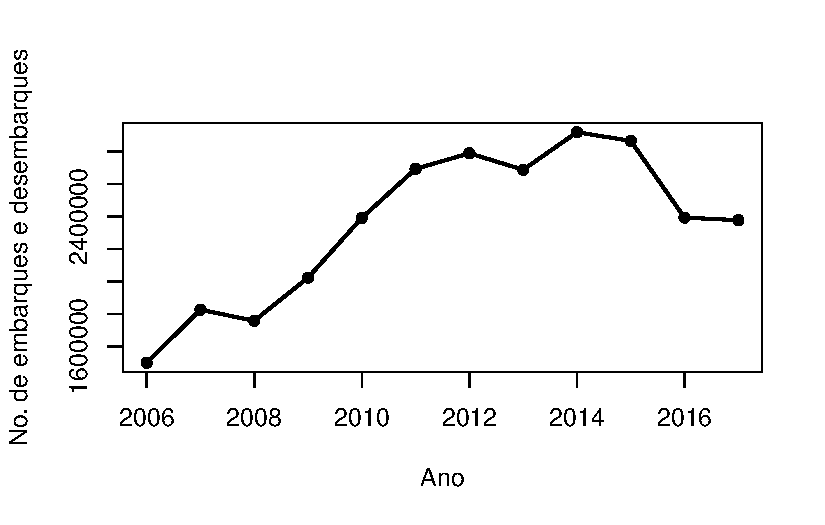
\includegraphics{intro_files/figure-pdf/unnamed-chunk-1-1.pdf}

Ainda considerando a série acima, seja \(x_t\) o número de embarques e
desembarques registrado no ano \(t\). A figura abaixo mostra o diagrama
de disperão entre \(x_t\) e \(x_{t-1}\), de onde é possível observar a
correlação positiva, estimada em 0,86.

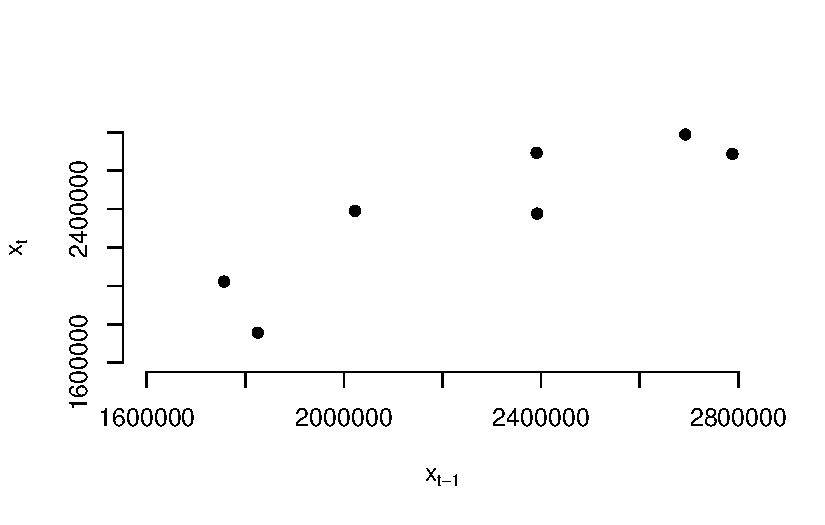
\includegraphics{intro_files/figure-pdf/unnamed-chunk-2-1.pdf}

De posse desses resultados, pode-se imaginar um primeiro modelo, no qual
a relação entre o presente e o passado imediato é ditado por uma
regressão linear simples, gerando a equação

\[\hat{x}_t = 7,589\times 10^5 +0,7109 x_{t-1}.\] Sabendo que
\(x_{2017}=2.376.505\), uma previsão para 2018 seria
\(\hat{x}_{2018}=2.448.357\). O valor observado em 2018 foi 2.572.159,
gerando um erro de previsão igual a \(x_{2018}-\hat{x}_{2018}=195.654\)
embarques e desembarques domésticos.

\hypertarget{exemplos-de-suxe9ries-temporais}{%
\section{Exemplos de séries
temporais}\label{exemplos-de-suxe9ries-temporais}}

\hypertarget{eletrocardiograma}{%
\subsection{Eletrocardiograma}\label{eletrocardiograma}}

\begin{Shaded}
\begin{Highlighting}[]
\FunctionTok{ts.plot}\NormalTok{(ECG)}
\end{Highlighting}
\end{Shaded}

\begin{figure}

\begin{minipage}[t]{\linewidth}

{\centering 

\raisebox{-\height}{

\includegraphics{intro_files/figure-pdf/unnamed-chunk-4-1.pdf}

}

\caption{1800 medidas da taxa cardíaca instantânea, em batidas por
minuto, de um indivíduo.}

}

\end{minipage}%

\end{figure}

\hypertarget{produto-interno-brupo-brasileiro}{%
\subsection{Produto Interno Brupo
Brasileiro}\label{produto-interno-brupo-brasileiro}}

\begin{Shaded}
\begin{Highlighting}[]
\FunctionTok{ts.plot}\NormalTok{(PIB)}
\end{Highlighting}
\end{Shaded}

\begin{figure}

\begin{minipage}[t]{\linewidth}

{\centering 

\raisebox{-\height}{

\includegraphics{intro_files/figure-pdf/unnamed-chunk-5-1.pdf}

}

\caption{PIB entre 1967 e 2014 corrigidos pelo valor do dólar em
4/2015.}

}

\end{minipage}%

\end{figure}

\hypertarget{mortes-por-doenuxe7as-pulmonares-no-reino-unido}{%
\subsection{Mortes por doenças pulmonares no Reino
Unido}\label{mortes-por-doenuxe7as-pulmonares-no-reino-unido}}

\begin{Shaded}
\begin{Highlighting}[]
\FunctionTok{ts.plot}\NormalTok{(ldeaths)}
\end{Highlighting}
\end{Shaded}

\begin{figure}

\begin{minipage}[t]{\linewidth}

{\centering 

\raisebox{-\height}{

\includegraphics{intro_files/figure-pdf/unnamed-chunk-6-1.pdf}

}

\caption{PIB entre 1967 e 2014 corrigidos pelo valor do dólar em
4/2015.}

}

\end{minipage}%

\end{figure}

\bookmarksetup{startatroot}

\hypertarget{suxe9ries-estacionuxe1rias}{%
\chapter{Séries Estacionárias}\label{suxe9ries-estacionuxe1rias}}

Uma coleção do tipo \(\{x(t),t\in\mathcal{T}\}\),
\(\mathcal{T}\subseteq \mathbb{R}\), onde \(x(t)\) é uma variável
aleatória para cada \(t\) fixado, é denominada processo estocástico.

Um processo estocástico é dito ser fortemente estacionário se sua
distribuição é invariante ao índice. Portanto, para qualquer
\(t_1,\ldots,t_k\), a distribuição de \(x(t_1),\ldots,x(t_k)\) é a mesma
de \(x(t_1+h),\ldots,x(t_k+h)\).

\begin{example}[]\protect\hypertarget{exm-serie_estacionaria_1}{}\label{exm-serie_estacionaria_1}

Se \(x(t)\sim \hbox{Normal}(0,1)\) e \(x(t)\) é independente de \(x(s)\)
para todo \(t\neq s\), então, para qualquer \(t_1,\ldots,t_k\),

\[\begin{align}P(x(t_1)<x_1,\ldots,x(t_k)<x_k)&=\prod_{i=1}^k P(x(t_i)<x_i)=\prod_{i=1}^k P(x(t_i+h)<x_i)\\&=P(x(t_1+h)<x_1,\ldots,x(t_k+h)<x_k)\end{align}\]
logo, \(\{x(t),t\in \mathbb{R}\}\) é um processo fortemente
estacionário. \(\blacksquare\)

\end{example}

\begin{theorem}[]\protect\hypertarget{thm-exm_estacionaria2}{}\label{thm-exm_estacionaria2}

Seja \(\{x(t),t\in\mathbb{N}\}\) um processo estocástico com
\[x(t)= x_{(t-1)}+\varepsilon_t,\;\;\varepsilon_t\sim\hbox{Normal}(0,1),\]
para \(t=1,2,\ldots\) com a condição de que
\(x_0\sim\hbox{Normal}(0,1)\) e que
\(Cov(\varepsilon_t,\varepsilon_s)=0\;\;\forall s\neq t\). Então,
\[x_t=x_{t-1}+\varepsilon_{t}=\cdots=x_0+\sum_{j=1}^t\varepsilon_t\sim\hbox{Normal}(0,t+1).\]
Como \(x_t\sim\hbox{Normal}(0,t+1)\) e, para qualquer \(h>0\),
\(x_{t+h}\sim\hbox{Normal}(0,t+h+1)\), temos que este processo não é
fortemente estacionário. \(\blacksquare\)

\end{theorem}

\begin{definition}[]\protect\hypertarget{def-fracamente}{}\label{def-fracamente}

Um processo estocástico \(\{y_t\}\) é dito ser fracamente estacionário
(ou de segunda ordem) se \[\begin{align*}
    E(y_t)&=\mu,\\
    Var(y_t)&=\nu,\\ 
    Cov(y_t,y_s)&=E(y_ty_s)-E(y_t)E(y_s)=\gamma(t-s)
    \end{align*}\] onde \(\mu\) e \(\nu\) são constantes independentes
de \(t\) e \(\gamma(t-s)\) depende de \(t\) e \(s\) somente através da
diferença \(|t-s|\). \(\blacksquare\)

\end{definition}

\begin{example}[]\protect\hypertarget{exm-fracamente1}{}\label{exm-fracamente1}

Considere o processo estocástico \(\{x(t),t\in\mathbb{N}\}\), onde
\[x(t) = \varepsilon(t) +\frac{1}{2}\varepsilon(t-1)
\] onde \(\varepsilon(t)\sim\hbox{Normal}(0,\nu)\) para \(t=1,\ldots\),
\(\varepsilon(t)\) é independente de \(\varepsilon(s)\) para todo
\(s\neq t\) e \(\varepsilon(0)=0\). Então: \[\begin{align}
E(x(t))&=E(\varepsilon(t))+\frac{1}{2}E(\varepsilon(t-1))=0\\
Var(x(t))&=Var(\varepsilon(t))+\frac{1}{4}Var(\varepsilon(t-1))=\frac{5}{4}\nu
\end{align}
\] e \[\begin{align}
          Cov(x(t),x(t+h))&=Cov\left(\varepsilon(t)+\frac{1}{2}\varepsilon(t-1),\varepsilon(t+h)+\frac{1}{2}\varepsilon(t+h-1)\right)\\
          &=Cov\left(\varepsilon(t),\varepsilon(t+h)\right)+\frac{1}{2}Cov\left(\varepsilon(t),\varepsilon(t+h-1)\right)\\
          &+\frac{1}{2}Cov\left(\varepsilon(t-1),\varepsilon(t+h)\right)+\frac{1}{4}Cov\left(\varepsilon(t-1),\varepsilon(t+h-1)\right)\\
          &=\left\{ \begin{array}{ll}
          \frac{4}{5}\nu,&\; h = 0 \\         
          \frac{1}{2}\nu,&\; |h|=1,\\
          0,&\;\hbox{caso contrário.}
          \end{array} \right.
    \end{align}\] Portanto, o processo é fracamente estacionáriao.
\(\blacksquare\)

\end{example}

Quando \(\mathcal{T}=\{t\in D\subseteq \mathbb{Z}\}\), utiliza-se a
notação \(x(t)=x_t\). Além disso, se \(t\) pode ser interpretado como
tempo, \(x_t\) é uma série temporal. Uma série temporal é dita ser
estacionária se ela é fracamente estacionária e o mesmo princípio se
aplica nessas notas de aula.

\hypertarget{processo-estacionuxe1rio-erguxf3dico}{%
\section{Processo estacionário
ergódico}\label{processo-estacionuxe1rio-erguxf3dico}}

Seja \(x_1,x_2,\ldots,x_n\) uma série temporal estacionária. Então, a
média \(\mu\) pode ser estimada por \(\bar{x}_n\), uma vez que
\(E(\bar{x})=\mu\). A variância essa estatística é

\[\begin{align}Var(\bar{x})&=Cov(\bar{x}_n,\bar{x}_n)=Cov\left(\sum_{i=1}^n \frac{x_i}{n},\sum_{j=1}^n\frac{x_j}{n}\right)=\frac{1}{n^2}\sum_{i=1}^n\sum_{j=1}^nCov(x_i,x_j)\\
&=\frac{1}{n^2}\left[\sum_{i=1}^nCov(x_i,x_i)+2\sum_{i=1}^n\sum_{j\neq i}Cov(x_i,x_j)\right]\\
&=\frac{1}{n^2}\left[n\nu+2\sum_{h=1}^{n-1}(n-h)\gamma(h)\right]=\frac{\nu}{n}+\frac{2}{n}\sum_{h=1}^{n-1}\left(1-\frac{h}{n}\right)\gamma(h)
\end{align}\]

Note que, diferente do caso independente e identicamente distribuído,
\(\bar{x}\) não é necessariamente um estimador adequado, conforme pode
ser constatado no exemplo abaixo.

\begin{example}[]\protect\hypertarget{exm-estationario_nao_ergodico}{}\label{exm-estationario_nao_ergodico}

Seja \(x_t\) um processo onde \(x_0\sim\hbox{Normal}(0,\nu)\) e
\(x_t=x_0\) para todo \(t>0\). Como

\[\begin{align}
E(x_t)&=E(E(x_t|x_0))=E(x_0)=0\\
Var(x_t)&=E(Var(x_t|x_0))+Var(E(x_t|x_0))=E(0)+Var(x_0)=\nu\\
Cov(x_t,x_{t-h})&=E( Cov(x_t,x_{t-h}|x_0))+Cov( E(x_t|x_0),E(x_{t-h}|x_0))\\
&=E(0)+Cov(x_0,x_0)=Var(x_0)=\nu
\end{align}\] e, portanto, o processo é fracamente estacionário.
Contudo,
\[Var(\bar{x})=\frac{\nu}{n}+\frac{2}{n}\sum_{h=1}^{n-1}\left(1-\frac{h}{n}\right)\nu=\nu,\]
portanto, o erro padrão não decai com o aumento do tamanho da amostra.

\(\blacksquare\)

\end{example}

A partir do exemplo acima, fica claro que \(\bar{x}\) nem sempre será um
estimador adequado para uma série estacionária.

\begin{definition}[]\protect\hypertarget{def-ergodica}{}\label{def-ergodica}

Uma série temporal estacionária é dita ser ergódica para a média se
\[\sum_{i=1}^n\frac{x_1}{n}\stackrel{p}{\rightarrow} \mu,\] quando
\(n\rightarrow\infty\).

\end{definition}

A partir deste momento será considerado que toda série temporal
estacionária é ergódica e, portanto \(\bar{x}\) é um estimador para
\(\mu\).

\begin{example}[]\protect\hypertarget{exm-estationario_nao_ergodico_conclusao}{}\label{exm-estationario_nao_ergodico_conclusao}

Considere novamente o processo no
(\textbf{estationario\_nao\_ergodico?}). Como \(\bar{x}_n=x_0\), tem-se
que, para \(\varepsilon>0\) arbitrário,
\(\bar{x}\sim\hbox{Normal}(0,\nu)\) e
\[P(|\bar{x}_n-0|>\varepsilon)=2P(x_0>\varepsilon)=2\int_{-\infty}^\varepsilon \frac{1}{\sqrt{2\pi\nu}}e^{-\frac{y^2}{2\nu}}d\nu>\frac{1}{2}\]
logo, \(\bar{x}\) não converge em probabilidade para \(0\) e, portanto,
o processo não é ergódico na média. \(\blacksquare\)

\end{example}

\hypertarget{ruuxeddo-branco}{%
\section{Ruído branco}\label{ruuxeddo-branco}}

\begin{definition}[]\protect\hypertarget{def-ruido_branco}{}\label{def-ruido_branco}

A série estacionária \(x_t\) é dita ser um ruído branco se \(E(x_t)=0\),
\(Var(x_t)=\nu\) e \[\begin{equation}
        Cov(x_t,x_s)=0,
        \end{equation}\] para todo \(t\neq s\). \(\blacksquare\)

\end{definition}

É imediato que o ruído branco é uma série temporal estacionária. Além
disso, pela Desigualdade de Chebyshev, para qualquer \(\varepsilon>0\),

\[P\left(|\bar{x}_n|\geq\varepsilon\right)\leq \frac{E(\bar{x}_n^2)}{\varepsilon^2}=\frac{Var(\bar{x}_n)}{\varepsilon^2}=\frac{\nu}{n\varepsilon^2}\]
logo \(\lim_{n}P(|\bar{x}_n|\leq \varepsilon)=0\) e
\(\bar{x}_n\stackrel{p}{\rightarrow}0\). Portanto, o ruído branco é
ergódico.

Considere agora a série temporal \(y_t=\mu+x_t\), onde \(x_t\) é um
ruído branco. Então
\[\bar{y}_n=\mu+\bar{x}_n\stackrel{p}{\rightarrow}\mu\] e \(\bar{y}_n\)
é um estimador para \(\mu\).

Em certos momentos, será considerado que \(x_t\) e \(x_s\), para todo
\(t\neq s\) são independentes (essa é uma condição mais forte, pois
implica em \(Cov(x_t,x_s)=0\)). Esse processo é denominado ruído branco
independente.

Por último, também será considerado a possibilidade de que
\(x_t\sim\hbox{Normal}(0,\nu)\), com \(x_t\) e \(x_s\) indepentens para
todo \(t\neq s\). Esse processo será denominado é denominado ruído
branco gaussiano.

\bookmarksetup{startatroot}

\hypertarget{defasagens-e-autocorrelauxe7uxe3o}{%
\chapter{Defasagens e
autocorrelação}\label{defasagens-e-autocorrelauxe7uxe3o}}

\hypertarget{gruxe1fico-de-defasagens}{%
\section{Gráfico de Defasagens}\label{gruxe1fico-de-defasagens}}

Denomina-se por \textbf{defasagem} \(h\) (\emph{lag}, em inglês), um
atraso em \(h\) nos índices da série temporal. A tabela abaixo ilustra
algumas defasagens para a série \(x_1,\ldots,x_5\)

\begin{longtable}[]{@{}llll@{}}
\toprule\noalign{}
Série original & \(h=1\) & \(h=2\) & \(h=3\) \\
\midrule\noalign{}
\endhead
\bottomrule\noalign{}
\endlastfoot
\(x_1\) & & & \\
\(x_2\) & \(x_1\) & & \\
\(x_3\) & \(x_2\) & \(x_1\) & \\
\(x_4\) & \(x_3\) & \(x_2\) & \(x_1\) \\
\(x_5\) & \(x_4\) & \(x_3\) & \(x_2\) \\
\end{longtable}

Conforme dito anteriormente, a existência de uma estrutura de
dependência entre \(x_t\) e \(x_{t-h}\) permite que a série observada
seja utilizada para realizar previsões. Uma ferramenta exploratória
interessante para analisar esse tipo de estrutura é gráfico de
defasagens (no inglês \emph{lag plot}). Trata-se de um diagrama de
dispersão entre a série original e a série defasada, para algum \(h\)
fixado. Abaixo apresenta-se a série de embarques e desembraques no
aeroporo Eduardo Gomes para as 4 primeiras defasagens. Os números
representam a ordem (temporal) dos pares do diagrama e a linha cinza
pontilha é a reta \(y=x\).

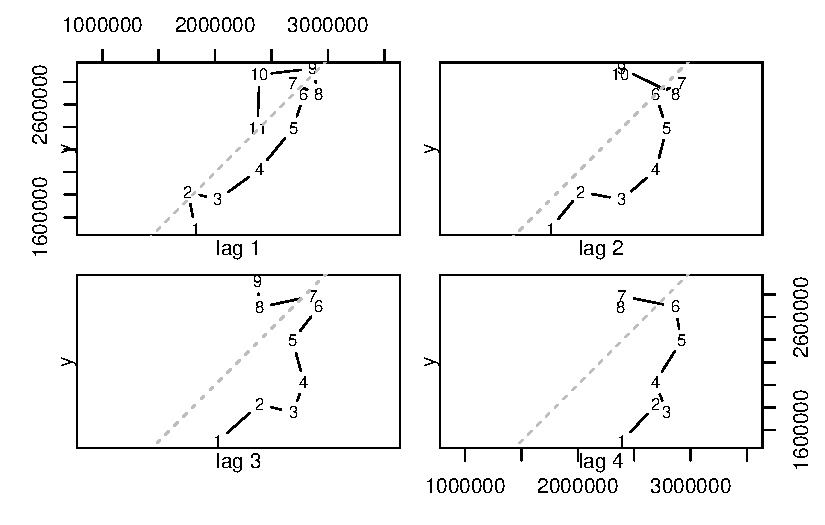
\includegraphics{acf_files/figure-pdf/unnamed-chunk-1-1.pdf}

Abaixo, a figura mostra o gráfico de defasagens para \(h=1,2,3,12\)
considerando a série de mortes por doenças pulmonares no Reino Unido.

\includegraphics{acf_files/figure-pdf/unnamed-chunk-2-1.pdf}

\hypertarget{a-funuxe7uxe3o-de-autocorrelauxe7uxe3o}{%
\section{A função de
autocorrelação}\label{a-funuxe7uxe3o-de-autocorrelauxe7uxe3o}}

\begin{definition}[]\protect\hypertarget{def-autocovariancia}{}\label{def-autocovariancia}

A função de autocovariância da série temporal \(x_t\) é dada por
\[\begin{equation}
          \gamma(s,t) = Cov(x_t,x_s)=E\left[(x_t-\mu_t)(x_s-\mu_s)\right],
        \end{equation}\] para todo \(s,t\) com \(\mu_j=E(y_j)\) e sua
respectiva função de autocorrelção é dada por \[\begin{equation}
        \rho(s,t)=\frac{\gamma(s,t)}{\sqrt{\gamma(s,s)\gamma(t,t)}}
        \end{equation}\]

\end{definition}

\begin{example}[]\protect\hypertarget{exm-acf1}{}\label{exm-acf1}

Considere a série temporal
\[x_t= x_{t-1}+\varepsilon_t,\;\;\varepsilon_t\sim\hbox{Normal}(0,1),\]
para \(t=1,2,\ldots\) com a condição de que \(x_0=0\) e que
\(Cov(\varepsilon_t,\varepsilon_s)=0\;\;\forall s\neq t\). É imediato
que \[\begin{equation}
    x_{t}=\sum_{j=1}^{t}\varepsilon_{j},
    \end{equation}\] o que implica em \(x_t\sim\hbox{Normal}(0,t)\).
Portanto, \[\begin{align}
        E(x_t)&=0\\
        Var(x_t)&=t.
        \end{align}\] Além disso, \[\begin{align*}
    \gamma(t,t-h)&=Cov(x_t,x_{t-h})=Cov\left(\sum_{i=1}^{t}\varepsilon_{i},\sum_{j=1}^{t-h}\varepsilon_{j}\right)\\
    &=\sum_{i=1}^{t}\sum_{j=1}^{t-h}Cov\left(\varepsilon_{i},\varepsilon_{j}\right)=\sum_{i=1}^{t-h}Cov(\varepsilon_i,\varepsilon_i)\\
    &=t-h
    \end{align*}\] e \[\begin{equation}
    \rho(t,t-h)=\frac{\gamma(t,t-h)}{\sqrt{\gamma(t,t)\gamma(t-h,t-h)}}=\frac{t-h}{\sqrt{t(t-h)}}=\sqrt{1-\frac{h}{t}}
    \end{equation}\] A figura abaixo mostra o gráfico da função de
autocorrelação desse processo, considerando uma série de tamanho 100.
Note que a série é mais dependente dos valores atuais, embora ainda
possua uma autocorrelação alta para defasagens elevadas.

\begin{Shaded}
\begin{Highlighting}[]
\FunctionTok{curve}\NormalTok{( }\FunctionTok{sqrt}\NormalTok{(}\DecValTok{1}\SpecialCharTok{{-}}\NormalTok{x}\SpecialCharTok{/}\DecValTok{100}\NormalTok{),}\DecValTok{0}\NormalTok{,}\DecValTok{99}\NormalTok{, }\AttributeTok{xlab=} \StringTok{\textquotesingle{}Defasagem\textquotesingle{}}\NormalTok{, }\AttributeTok{ylab =} \StringTok{\textquotesingle{}Autocorrelação\textquotesingle{}}\NormalTok{)}
\end{Highlighting}
\end{Shaded}

\begin{figure}

\begin{minipage}[t]{\linewidth}

{\centering 

\raisebox{-\height}{

\includegraphics{acf_files/figure-pdf/unnamed-chunk-3-1.pdf}

}

\caption{Função de autocorrelação do Exemplo Example~\ref{exm-acf1},
para t=100}

}

\end{minipage}%

\end{figure}

\(\blacksquare\)

\end{example}

Para uma série estacionária, tem-se que \(E(x_t)=\mu\) para todo \(t\),
logo \[\begin{equation}
        \gamma(t-s) = Cov(y_t,y_s)=E\left[(y_t-\mu)(y_s-\mu)\right].
\end{equation}\] Fazendo \(h=t-s\), tem-se \[\begin{equation}
            \gamma(h)=Cov(y_t,y_{t-h}).
        \end{equation}\]

A função de autocorrelação (ACF) para um processo estacionário é
\[\begin{equation}
                \rho(h)=\frac{\gamma(h)}{\gamma(0)}
\end{equation}\] e ela mede a dependência linear entre \(y_t\) e os
valores defasados da série.Sempre será verdade que \(\rho\in[-1,1]\),
\(\rho(h)=\rho(-h)\) e, se \(y_{t+h}\) é independente de \(y_t\), então
\(\rho(h)=0\).

\begin{example}[]\protect\hypertarget{exm-acf2}{}\label{exm-acf2}

Considere a série temporal \[\begin{align}
    x_t = \varepsilon_t +\frac{1}{2}\varepsilon_{t-1} \label{exer1}
    \end{align}\] onde \(\varepsilon_t\sim\hbox{Normal}(0,\nu)\) para
\(t=1,\ldots\), \(\varepsilon_t\) é independente de \(\varepsilon_s\)
para todo \(s\neq t\) e \(\varepsilon_0=0\). Como \[\begin{align}
    E(x_t)&=E(\varepsilon_t)+\frac{1}{2}E(\varepsilon_{t-1})=0\\
    Var(x_t)&=Var(\varepsilon_t)+\frac{1}{4}Var(\varepsilon_{t-1})=\frac{5}{4}\nu\\
    \gamma(h)&=\left\{ \begin{array}{ll}
    \frac{5}{4}\nu,&\; h = 0 \\       
    \frac{1}{2}\nu,&\; |h|=1,\\
    0,&\;\hbox{caso contrário.}
    \end{array} \right.
    \end{align}
\]\\
tem-se que, \[\begin{align}
    \rho(h)&=\frac{\gamma(h)}{\gamma(0)}=\left\{ \begin{array}{ll}
    1,&\; h = 0 \\        
    \frac{2}{5},&\; |h|=1,\\
    0,&\;\hbox{caso contrário.}
    \end{array} \right.
    \end{align}\] \(\blacksquare\)

\end{example}

\begin{example}[]\protect\hypertarget{exm-acf_ruido_branco}{}\label{exm-acf_ruido_branco}

Seja \(x_t\) um ruído branco. Então \[\gamma(h)=\nu I(h=0),\] e
\[\rho(h)=\frac{\gamma(h)}{\gamma(0)}=I(h=0),\] onde \(I(A)\) é a função
indicadora da ocorrência do evento \(A\).

\end{example}

\hypertarget{a-funuxe7uxe3o-de-autocorrelauxe7uxe3o-estimada-e-o-correlograma}{%
\section{A função de autocorrelação estimada e o
correlograma}\label{a-funuxe7uxe3o-de-autocorrelauxe7uxe3o-estimada-e-o-correlograma}}

Considere uma série temporal \(x_1,\ldots,x_n\). Supondo que ela é
proveniente de uma série estacionária (ergódico), pode-se estimar
\(\gamma(h)\) pelo método da substituição: \[\begin{align}
                        \widehat{\gamma(h)}&=\frac{1}{n}\sum_{i=1}^{n-h}\left(x_{i+h} - \bar{x}\right)\left(x_{i} - \bar{x}\right)
                        \end{align}\] e \(\rho\) por\\
\[\begin{equation}
        \hat{\rho}(h)=\frac{\hat{\gamma}(h)}{\hat{\gamma}(0)}
        \end{equation}\]

É importante notar que tanto \(\gamma(h)\) quanto \(\rho(h)\) são
invariantes a transformações de locação. Por exemplo, seja \(\gamma(h)\)
a função de autocovariância de \(x_t\) e considere \(y_t=x_t+a\). Então
\(E(y_t)=\mu+a\) e
\[E[(y_t-\mu-a)(y_{t-h}-\mu-a)]=E[(x_t-\mu)(x_{t-h}-\mu)]=\gamma(h).\]

O correlograma é um gráfico cartesiano construído a partir dos pontos
\((h, \hat{\rho})\). A partir de cada ponto é desenhada uma linha,
semelhante a um gráfico de barras. Como \(\hat{\rho}(0)=1\), a
implementação desta função em softwares estatísticos pode variar com
\(h=0\) ou em 1. Por exemplo, a função \texttt{acf} do pacote
\texttt{stats} começa na defasagem 0, enquanto a função \texttt{Acf} do
pacote \texttt{forecast} (ou ainda a \texttt{acf} do pacote
\texttt{TSA}) começam na defasagem 1.

\begin{example}[]\protect\hypertarget{exm-afogamentos}{}\label{exm-afogamentos}

A série abaixo representa o número anual de óbitos por afogamento na
cidade de Manaus, entre 1996 e 2021. Os dados foram obtidos do
Ministério da Saúde (http://tabnet.datasus.gov.br/), considerando o
código internacional de doenças (CID10) W70 - Afogamento e submersão
conseqüentes a queda dentro de águas naturais.

\begin{Shaded}
\begin{Highlighting}[]
\NormalTok{url }\OtherTok{\textless{}{-}} \StringTok{\textquotesingle{}https://docs.google.com/spreadsheets/d/13MdzvZB5U85MkLy97ZRytkylikJu7rJoC1WL0XjKw{-}c/edit?usp=sharing\textquotesingle{}}

\FunctionTok{require}\NormalTok{(data.table)}
\NormalTok{dados }\OtherTok{\textless{}{-}} \FunctionTok{fread}\NormalTok{(url)}
\NormalTok{afogamentos }\OtherTok{\textless{}{-}} \FunctionTok{ts}\NormalTok{( dados[,}\DecValTok{2}\NormalTok{], }\AttributeTok{start =} \DecValTok{1996}\NormalTok{)}
\end{Highlighting}
\end{Shaded}

\begin{Shaded}
\begin{Highlighting}[]
\FunctionTok{ts.plot}\NormalTok{(afogamentos, }\AttributeTok{lwd =} \DecValTok{2}\NormalTok{, }\AttributeTok{main =} \StringTok{\textquotesingle{}\textquotesingle{}}\NormalTok{, }\AttributeTok{xlab =} \StringTok{\textquotesingle{}Ano\textquotesingle{}}\NormalTok{, }\AttributeTok{ylab =} \StringTok{\textquotesingle{}No. óbitos por afogamento\textquotesingle{}}\NormalTok{)}
\end{Highlighting}
\end{Shaded}

\begin{figure}

\begin{minipage}[t]{\linewidth}

{\centering 

\raisebox{-\height}{

\includegraphics{acf_files/figure-pdf/unnamed-chunk-5-1.pdf}

}

\caption{Número anual de óbitos por afogamento em Manaus.}

}

\end{minipage}%

\end{figure}

A figura abaixo mostra o correlograma dessa série. Observe que as
autocorrelações amostrais observadas são baixas. Esse tipo de
comportamento é esperado em um ruído branco. Como a série não oscila em
torno de zero, um modelo razoável seria \[y_t=\mu+\varepsilon_t,\] onde
\(\varepsilon_t\) é um ruído branco. Nesse caso, \(\bar{y}_n=1,88\) é
uma estimativa para \(\mu\).

\begin{Shaded}
\begin{Highlighting}[]
\FunctionTok{acf}\NormalTok{(afogamentos, }\AttributeTok{lwd =} \DecValTok{2}\NormalTok{, }\AttributeTok{main =} \StringTok{\textquotesingle{}\textquotesingle{}}\NormalTok{, }\AttributeTok{xlab =} \StringTok{\textquotesingle{}Defasagem\textquotesingle{}}\NormalTok{, }\AttributeTok{ylab =} \StringTok{\textquotesingle{}Autocorrelação\textquotesingle{}}\NormalTok{)}
\end{Highlighting}
\end{Shaded}

\begin{figure}

\begin{minipage}[t]{\linewidth}

{\centering 

\raisebox{-\height}{

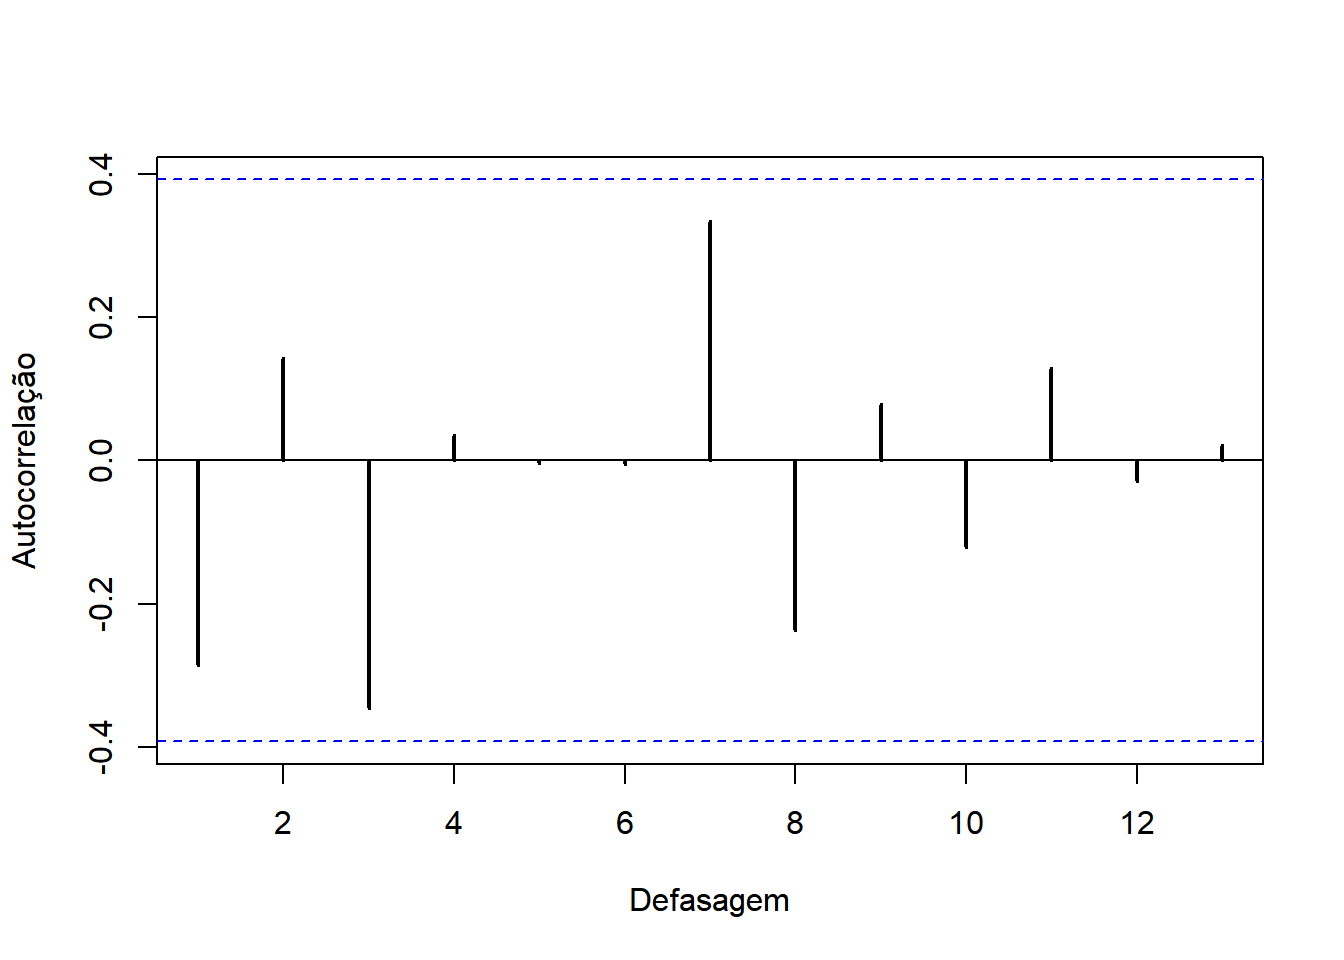
\includegraphics{acf_files/figure-pdf/fig-acf_afogamentos-1.pdf}

}

\caption{\label{fig-acf_afogamentos}Correlograma para o número anual de
óbitos por afogamento em Manaus.}

}

\end{minipage}%

\end{figure}

\(\blacksquare\)

\end{example}

Sem perda de generalidade, assuma que \(x_t\) é um processo estacionário
com \(\mu=0\). Para uma defasagem \(h>0\), considere a hipótese
\(H_0:\rho(h)=0\). Sob \(H_0\), o processo estacionário é um ruído
branco e a distribuição da função de autocorrelação amostral é
\(N(0,1/n)\). Portanto, uma região de rejeição ao níve de 5\% de
significância para um teste baseado nessa distribuição é\\
\[R={\hat{\rho}(h): \hat{\rho}(h)|>\frac{2}{\sqrt{n}},\] Este é o valor
da linha pontilhada que aparece no correlograma na
Figure~\ref{fig-acf_afogamentos}.

\hypertarget{testes-para-a-autocorrelauxe7uxe3o}{%
\section{Testes para a
autocorrelação}\label{testes-para-a-autocorrelauxe7uxe3o}}

Na seção anterior mostrou-se como testar \(H_0:\rho(h)=0\), para um
\(h\) fixado. Como várias autocorrelações para diferentes defasagens são
avaliadas simultaneamente, o correto seria testar
\(H_0: \rho(h)=0\;\;\forall h=1,\ldots,q\), onde \(q\) é o valor máximo
da defasagem a ser testado. Considerando a região de rejeição dada
anteriormente, pela desigualdade de Bonferroni,

\[\begin{align}P(\hbox{Rejeitar }H_0|H_0\hbox{ é verdadeira})&=P\left(\cup_{h=1}^q\left\{ \hat{\rho}(h)>\frac{2}{\sqrt{n}}\right\}| H_0\hbox{ é verdade}\right)\\
&\leq \sum_{h=1}^qP\left( \hat{\rho}(h)>\frac{2}{\sqrt{n}}| H_0\hbox{ é verdade}\right)\\ &<q\alpha\end{align}\]

Portanto, a probabilidade de cometer o erro tipo 1 pode aumentar na
medida que testamos mais de uma defasagem.

Como alternativa, considere a mesma hipótese nula. Se todas as
autocorrelaçãoes, de defasagens 1 até \(q\), são baixas, não há
evidências contra \(H_0\). Com esse espírito o teste de Ljung-Box (1978)
utiliza a estatística
\[Q_{LB}=n(n+2)\sum_{h=1}^q \frac{\hat{\rho}(h)^2}{n-h}\] e rejeita
\(H_0\) se \(Q_{LB}>\chi^2_{1-\alpha,q}\), onde \(\chi^2_{\lambda,n}\) é
o quantil \(\lambda\) da distribuição \(\chi^2_n\).

O teste de Box-Pierce (1970) possui o mesmo objetivo e tem a mesma regra
de decisão, mudando apenas a estatística de teste para

\[Q_{BP}=n\sum_{h=1}^q \frac{\hat{\rho}(h)^2}{n-h}.\]

\begin{example}[]\protect\hypertarget{exm-afogamentos_testes}{}\label{exm-afogamentos_testes}

Para a série de óbitos anuais por afogamentos em Manaus, tem-se que os
teste Ljung-Box e Box-Pierce não rejeitam a hipótese de ruído branco.

\begin{Shaded}
\begin{Highlighting}[]
\FunctionTok{Box.test}\NormalTok{(afogamentos, }\AttributeTok{type =} \StringTok{\textquotesingle{}Ljung{-}Box\textquotesingle{}}\NormalTok{)}
\end{Highlighting}
\end{Shaded}

\begin{verbatim}

    Box-Ljung test

data:  afogamentos
X-squared = 2.2888, df = 1, p-value = 0.1303
\end{verbatim}

\begin{Shaded}
\begin{Highlighting}[]
\FunctionTok{Box.test}\NormalTok{(afogamentos, }\AttributeTok{type =} \StringTok{\textquotesingle{}Box{-}Pierce\textquotesingle{}}\NormalTok{)}
\end{Highlighting}
\end{Shaded}

\begin{verbatim}

    Box-Pierce test

data:  afogamentos
X-squared = 2.0345, df = 1, p-value = 0.1538
\end{verbatim}

\(\blacksquare\)

\end{example}

\bookmarksetup{startatroot}

\hypertarget{criando-suxe9ries-no-r}{%
\chapter{\texorpdfstring{Criando séries no
\texttt{R}}{Criando séries no R}}\label{criando-suxe9ries-no-r}}

Esta seção tem por objetivo mostrar algumas funções em \texttt{R} para a
criação e análise exploratória de séries temporais.

\hypertarget{a-classe-ts}{%
\section{\texorpdfstring{A classe
\texttt{ts}}{A classe ts}}\label{a-classe-ts}}

Para todos os efeitos, uma série temporal é um vetor numérico. O vetor
abaixo armazena o número de nascidos vivos por mês na cidade de Manaus
em 2021, sendo \texttt{x{[}1{]}} o mês de janeiro e assim
sucessivamente.

\begin{Shaded}
\begin{Highlighting}[]
\NormalTok{x }\OtherTok{\textless{}{-}} \FunctionTok{c}\NormalTok{( }\DecValTok{3043}\NormalTok{, }\DecValTok{2902}\NormalTok{, }\DecValTok{3166}\NormalTok{, }\DecValTok{3014}\NormalTok{, }\DecValTok{3095}\NormalTok{, }\DecValTok{2955}\NormalTok{, }\DecValTok{3087}\NormalTok{, }\DecValTok{3141}\NormalTok{,}
\DecValTok{3129}\NormalTok{, }\DecValTok{3096}\NormalTok{, }\DecValTok{3191}\NormalTok{, }\DecValTok{3222}\NormalTok{)}
\end{Highlighting}
\end{Shaded}

Por sua vez, o gráfico da série temporal pode ser construído utilizando
a função \texttt{plot}, com o argumento
\texttt{type=\textquotesingle{}l\textquotesingle{}}.

\begin{Shaded}
\begin{Highlighting}[]
\FunctionTok{plot}\NormalTok{(x, }\AttributeTok{type =} \StringTok{\textquotesingle{}l\textquotesingle{}}\NormalTok{)}
\end{Highlighting}
\end{Shaded}

\begin{figure}[H]

{\centering \includegraphics{ts_window_date_files/figure-pdf/unnamed-chunk-2-1.pdf}

}

\end{figure}

Contudo, é útil construir a série temporal como um objeto da classe
\texttt{ts}. Tal função possui dois argumentos importantes:

\begin{itemize}
\item
  \texttt{frequency}: representa o número de observações por unidade de
  tempo. Por exemplo, se tempo está sendo contado em anos, mas o dados
  são mensais, então \texttt{frequency=12}; se os dados forem
  trimestrais, \texttt{frequency=4} e assim por diante.
\item
  \texttt{start}: representa o tempo da primeira observação. Pode ser
  representado por um único número ou por um vetor de comprimento dois.
  Esse último caso só é utilizado quando \texttt{frequency} é diferente
  de 1 e representa a ordem, em relação à frequência, da primeira
  observação. Por exemplo, com \texttt{frequency=12}, o vetor
  \texttt{start=c(1996,2)} implica que a primeira observação data de
  fevereiro de 1996.
\end{itemize}

No código abaixo, o vetor criado anteriormente é colocado com um objeto
\texttt{ts}

\begin{Shaded}
\begin{Highlighting}[]
\NormalTok{x }\OtherTok{\textless{}{-}} \FunctionTok{ts}\NormalTok{( x, }\AttributeTok{start =} \FunctionTok{c}\NormalTok{(}\DecValTok{2021}\NormalTok{,}\DecValTok{1}\NormalTok{), }\AttributeTok{frequency =} \DecValTok{12}\NormalTok{)}
\NormalTok{x}
\end{Highlighting}
\end{Shaded}

\begin{verbatim}
      Jan  Feb  Mar  Apr  May  Jun  Jul  Aug  Sep  Oct  Nov  Dec
2021 3043 2902 3166 3014 3095 2955 3087 3141 3129 3096 3191 3222
\end{verbatim}

\begin{Shaded}
\begin{Highlighting}[]
\FunctionTok{ts.plot}\NormalTok{(x)}
\end{Highlighting}
\end{Shaded}

\begin{figure}[H]

{\centering \includegraphics{ts_window_date_files/figure-pdf/unnamed-chunk-3-1.pdf}

}

\end{figure}

No gráfico acima, a parte decimal no eixo \(x\) representa a fração do
tempo entre de um ano (começando em 0 e acumulando 1/12 para cada mês
subsequente).

O gráfico pode ser customizado do mesmo modo que um \texttt{plot}.
Abaixo segue um exemplo.

\begin{Shaded}
\begin{Highlighting}[]
\FunctionTok{plot}\NormalTok{(x, }\AttributeTok{ylab =} \StringTok{\textquotesingle{}No. nascidos vivos mensal\textquotesingle{}}\NormalTok{, }\AttributeTok{lwd =} \DecValTok{2}\NormalTok{, }\AttributeTok{col =} \StringTok{\textquotesingle{}seagreen\textquotesingle{}}\NormalTok{)}
\end{Highlighting}
\end{Shaded}

\begin{figure}[H]

{\centering \includegraphics{ts_window_date_files/figure-pdf/unnamed-chunk-4-1.pdf}

}

\end{figure}

A função \texttt{start} retorna o início da série, \texttt{end} seu fim
e \texttt{frequency} o número de observações por unidade de tempo.
Observe o exemplo abaixo.

\begin{Shaded}
\begin{Highlighting}[]
\FunctionTok{start}\NormalTok{(x)}
\end{Highlighting}
\end{Shaded}

\begin{verbatim}
[1] 2021    1
\end{verbatim}

\begin{Shaded}
\begin{Highlighting}[]
\FunctionTok{end}\NormalTok{(x)}
\end{Highlighting}
\end{Shaded}

\begin{verbatim}
[1] 2021   12
\end{verbatim}

\begin{Shaded}
\begin{Highlighting}[]
\FunctionTok{frequency}\NormalTok{(x)}
\end{Highlighting}
\end{Shaded}

\begin{verbatim}
[1] 12
\end{verbatim}

A partir das informações acima, sabe-se a série \texttt{x} é mensal
(\texttt{frequency=12}), que sua primeira observação data de janeiro de
2021 e a última de dezembro de 2021.

\hypertarget{a-funuxe7uxe3o-window}{%
\section{\texorpdfstring{A função
\texttt{window}}{A função window}}\label{a-funuxe7uxe3o-window}}

A função \texttt{window} seleciona um subconjunto da série temporal.
Abaixo foram selecionados apenas os nascimentos entre Junho e Agosto e
este valores foram registrados no gráfico.

\begin{Shaded}
\begin{Highlighting}[]
\NormalTok{z }\OtherTok{\textless{}{-}} \FunctionTok{window}\NormalTok{(x, }\AttributeTok{start=}\FunctionTok{c}\NormalTok{(}\DecValTok{2021}\NormalTok{,}\DecValTok{6}\NormalTok{), }\AttributeTok{end =} \FunctionTok{c}\NormalTok{(}\DecValTok{2021}\NormalTok{,}\DecValTok{8}\NormalTok{))}

\FunctionTok{plot}\NormalTok{(x, }\AttributeTok{ylab =} \StringTok{\textquotesingle{}No. nascidos vivos mensal\textquotesingle{}}\NormalTok{, }\AttributeTok{lwd =} \DecValTok{2}\NormalTok{, }\AttributeTok{col =} \StringTok{\textquotesingle{}seagreen\textquotesingle{}}\NormalTok{)}
\FunctionTok{lines}\NormalTok{(z, }\AttributeTok{col =} \StringTok{\textquotesingle{}brown\textquotesingle{}}\NormalTok{, }\AttributeTok{lwd=} \DecValTok{2}\NormalTok{)}
\end{Highlighting}
\end{Shaded}

\begin{figure}[H]

{\centering \includegraphics{ts_window_date_files/figure-pdf/unnamed-chunk-6-1.pdf}

}

\end{figure}

\hypertarget{o-pacote-data.table}{%
\section{\texorpdfstring{O pacote
\texttt{data.table}}{O pacote data.table}}\label{o-pacote-data.table}}

Assim como números e textos possuem classes específicas, as datas no
ambiente \texttt{R} também possuem sua própria classe, denominada
\texttt{Date}.

\begin{Shaded}
\begin{Highlighting}[]
\CommentTok{\# 3 de agosto de 1998 (formato americano)}
\NormalTok{x }\OtherTok{\textless{}{-}} \StringTok{\textquotesingle{}1998/8/3\textquotesingle{}}
\FunctionTok{as.Date}\NormalTok{(x)}
\end{Highlighting}
\end{Shaded}

\begin{verbatim}
[1] "1998-08-03"
\end{verbatim}

Para que o \texttt{R} entenda uma data fora do padrão americano, é
necessário passar o formado para o argumento \texttt{format}. Seguem
alguns exemplos:

\begin{Shaded}
\begin{Highlighting}[]
\CommentTok{\# 3 de agosto de 1998 (formato nacional)}
\NormalTok{x }\OtherTok{\textless{}{-}} \StringTok{\textquotesingle{}3/8/1998\textquotesingle{}}
\FunctionTok{as.Date}\NormalTok{(x, }\AttributeTok{format =} \StringTok{\textquotesingle{}\%d/\%m/\%Y\textquotesingle{}}\NormalTok{)}
\end{Highlighting}
\end{Shaded}

\begin{verbatim}
[1] "1998-08-03"
\end{verbatim}

\begin{Shaded}
\begin{Highlighting}[]
\NormalTok{x }\OtherTok{\textless{}{-}} \StringTok{\textquotesingle{}3{-}8{-}1998\textquotesingle{}}
\FunctionTok{as.Date}\NormalTok{(x, }\AttributeTok{format =} \StringTok{\textquotesingle{}\%d{-}\%m{-}\%Y\textquotesingle{}}\NormalTok{)}
\end{Highlighting}
\end{Shaded}

\begin{verbatim}
[1] "1998-08-03"
\end{verbatim}

\begin{Shaded}
\begin{Highlighting}[]
\CommentTok{\# agosto de 1998}
\NormalTok{x }\OtherTok{\textless{}{-}} \StringTok{\textquotesingle{}8/1998\textquotesingle{}}
\FunctionTok{as.Date}\NormalTok{(x, }\AttributeTok{format =} \StringTok{\textquotesingle{}\%m/\%Y\textquotesingle{}}\NormalTok{)}
\end{Highlighting}
\end{Shaded}

\begin{verbatim}
[1] NA
\end{verbatim}

Ao se trabalhar com fontes originais, é comum ter como unidade amostral
um evento com sua data registrada. Em geral, nosso objetivo é determinar
a quantidade de eventos dentro de dias, semanas, meses ou anos. O pacote
\texttt{data.table} permite lidar com esse problema de modo rápido,
criando um objeto deste tipo utilizando a função \texttt{fread}.

Para ilustrar, será utilizada a base de dados de acidentes com
aeronaves, mantida pela Força Aérea Brasileira, que registra diariamente
o número de acidentes com aeronaves.

\begin{Shaded}
\begin{Highlighting}[]
\FunctionTok{library}\NormalTok{(data.table)}
\NormalTok{url }\OtherTok{\textless{}{-}} \StringTok{\textquotesingle{}https://drive.google.com/uc?authuser=0\&id=1iYrnwXgmLK07x8b330aD73scOVruZEuz\&export=download\textquotesingle{}}

\NormalTok{aereo }\OtherTok{\textless{}{-}}  \FunctionTok{fread}\NormalTok{(url, }\AttributeTok{encoding =} \StringTok{\textquotesingle{}Latin{-}1\textquotesingle{}}\NormalTok{)}
\NormalTok{aereo}\SpecialCharTok{$}\NormalTok{ocorrencia\_dia }\OtherTok{\textless{}{-}} \FunctionTok{as.Date}\NormalTok{(aereo}\SpecialCharTok{$}\NormalTok{ocorrencia\_dia, }\StringTok{\textquotesingle{}\%d/\%m/\%Y\textquotesingle{}}\NormalTok{)}
\end{Highlighting}
\end{Shaded}

Um objeto do tipo \texttt{data.table} permite uma série de consultas. Em
geral, pode-se fazer \texttt{aereo{[}a,b,c{]}}, onde \texttt{a} é uma
consulta/função nas linhas, \texttt{b} nas colunas e \texttt{c} é um
agrupador. Uma excelente introdução pode ser vista em
\href{https://cran.r-project.org/web/packages/data.table/vignettes/datatable-intro.html}{Introduction
to data.table}.

Abaixo, foi selecionada a coluna de interesse \texttt{ocorrencia\_dia}.

\begin{Shaded}
\begin{Highlighting}[]
\NormalTok{fab\_dia }\OtherTok{\textless{}{-}}\NormalTok{ aereo[,}\StringTok{\textquotesingle{}ocorrencia\_dia\textquotesingle{}}\NormalTok{,]}
\FunctionTok{head}\NormalTok{(fab\_dia)}
\end{Highlighting}
\end{Shaded}

\begin{verbatim}
   ocorrencia_dia
1:     2023-04-05
2:     2023-06-24
3:     2023-06-27
4:     2023-06-30
5:     2023-06-25
6:     2023-06-23
\end{verbatim}

Ao utilizar o operador \texttt{.N} em \texttt{{[},.N,c{]}}, é retornado
o número de linhas que possuem o agrupamento em \texttt{c}. Abaixo, as
datas do banco são agrupadas por ano.

\begin{Shaded}
\begin{Highlighting}[]
\NormalTok{fab\_ano }\OtherTok{\textless{}{-}}\NormalTok{ fab\_dia[, .N, by}\OtherTok{=}\NormalTok{.(}\FunctionTok{year}\NormalTok{(ocorrencia\_dia))]}
\NormalTok{fab\_ano }\OtherTok{\textless{}{-}}\NormalTok{fab\_ano[ }\FunctionTok{order}\NormalTok{(year) ]}
\FunctionTok{head}\NormalTok{(fab\_ano)}
\end{Highlighting}
\end{Shaded}

\begin{verbatim}
   year   N
1: 2013 654
2: 2014 569
3: 2015 471
4: 2016 403
5: 2017 432
6: 2018 444
\end{verbatim}

Os comandos a seguir criam dois objetos do tipo \texttt{ts}, sendo um
para o número anual de acidentes e outro para o mensal

\begin{Shaded}
\begin{Highlighting}[]
\NormalTok{fab\_ano }\OtherTok{\textless{}{-}} \FunctionTok{ts}\NormalTok{( fab\_ano, }\AttributeTok{start =} \DecValTok{2013}\NormalTok{)}
\FunctionTok{plot}\NormalTok{(fab\_ano[,}\DecValTok{2}\NormalTok{], }\AttributeTok{lwd =} \DecValTok{2}\NormalTok{, }\AttributeTok{ylab =} \StringTok{\textquotesingle{}No. acidentes/ano\textquotesingle{}}\NormalTok{, }\AttributeTok{xlab =} \StringTok{\textquotesingle{}Ano\textquotesingle{}}\NormalTok{)}
\end{Highlighting}
\end{Shaded}

\begin{figure}[H]

{\centering \includegraphics{ts_window_date_files/figure-pdf/unnamed-chunk-12-1.pdf}

}

\end{figure}

\begin{Shaded}
\begin{Highlighting}[]
\NormalTok{fab\_mes }\OtherTok{\textless{}{-}}\NormalTok{ fab\_dia[, .N, by}\OtherTok{=}\NormalTok{.(}\FunctionTok{year}\NormalTok{(ocorrencia\_dia), }\FunctionTok{month}\NormalTok{(ocorrencia\_dia))]}

\NormalTok{fab\_mes }\OtherTok{\textless{}{-}}\NormalTok{fab\_mes[ }\FunctionTok{order}\NormalTok{(year, month ) ]}
\NormalTok{fab\_mes }\OtherTok{\textless{}{-}} \FunctionTok{ts}\NormalTok{( fab\_mes[,}\DecValTok{3}\NormalTok{], }\AttributeTok{start =} \FunctionTok{c}\NormalTok{(}\DecValTok{2013}\NormalTok{, }\DecValTok{1}\NormalTok{), }\AttributeTok{frequency =} \DecValTok{12}\NormalTok{)}
\FunctionTok{plot}\NormalTok{(fab\_mes, }\AttributeTok{lwd =} \DecValTok{2}\NormalTok{, }\AttributeTok{ylab =} \StringTok{\textquotesingle{}No. acidentes/mês\textquotesingle{}}\NormalTok{, }\AttributeTok{xlab =} \StringTok{\textquotesingle{}Ano\textquotesingle{}}\NormalTok{)}
\end{Highlighting}
\end{Shaded}

\begin{figure}[H]

{\centering \includegraphics{ts_window_date_files/figure-pdf/unnamed-chunk-12-2.pdf}

}

\end{figure}

\hypertarget{exercuxedcio}{%
\section{Exercício}\label{exercuxedcio}}

Exercício 1

A série abaixo contém a data dos óbitos maternos no Brasil a partir de
2010.

\begin{Shaded}
\begin{Highlighting}[]
\NormalTok{url }\OtherTok{\textless{}{-}} \StringTok{\textquotesingle{}https://drive.google.com/uc?authuser=0\&id=1tYFFT9L2iopKmBDUI3P8qNIRaOnMYj7d\&export=download\textquotesingle{}}
\end{Highlighting}
\end{Shaded}

Crie uma série temporal com o número de óbitos mensal e faça um gráfico.
Crie uma janela para colocar no gráfico o período da pandemia de
COVID-19.

\bookmarksetup{startatroot}

\hypertarget{revisuxe3o-sobre-o-modelo-linear}{%
\chapter{Revisão sobre o modelo
linear}\label{revisuxe3o-sobre-o-modelo-linear}}

\hypertarget{definiuxe7uxe3o}{%
\section{Definição}\label{definiuxe7uxe3o}}

Para \(i=1,\ldots,n\), considere o modelo linear abaixo:
\[y_i= \beta_0+\sum_{j=1}^{p-1}x_{i,j}+\varepsilon_i=\underbrace{ \left(1\;\;x_{i,1}\;\;\cdots\;\;x_{i,p-1}\right)}_\text{$\boldsymbol{f}'_i$}\underbrace{\left(\begin{array}{c}\beta_0 \\ \beta_1 \\ \vdots \\ \beta_{p-1} 
        \end{array}\right)}_\text{$\boldsymbol{\beta}$}+\varepsilon_i=\boldsymbol{f}'_i\boldsymbol{\beta}+\varepsilon_i,\]
onde \(x_i\) é fixado e \(\varepsilon\) é um ruído branco gaussiano.
Pela independência entre \(y_i\) e \(y_j\), pode-se fazer a seguinte
representação estocástica de \(\boldsymbol{y}\): \[\begin{equation}
        \boldsymbol{y}=\boldsymbol{F}'\boldsymbol{\beta} + \boldsymbol{\varepsilon},
        \end{equation}\] onde
\(\boldsymbol{\varepsilon}\sim\hbox{Normal}(\boldsymbol{0},\nu\textbf{I}_n)\)
e \(\boldsymbol{F}\) é uma matriz \(p\times n\) conhecida com
\(i\)-ésima coluna dada por \(\boldsymbol{f}_i\):

\[\boldsymbol{F}=\left(\boldsymbol{f}_1,\ldots,\boldsymbol{F}\right).\]

A função de verossimilhança é dada por \[\begin{align*}
    L(\boldsymbol{\beta},\nu)&\propto \left(\frac{1}{v}\right)^{\frac{T}{2}}\exp\left\{-\frac{1}{2\nu}(\boldsymbol{y}-\boldsymbol{F}'\boldsymbol{\beta})'(\boldsymbol{y}-\boldsymbol{F}'\boldsymbol{\beta}) \right\}\\
    &\propto \left(\frac{1}{v}\right)^{\frac{T}{2}}\exp\left\{-\frac{1}{2\nu}\left[(\boldsymbol{\beta}-\hat{\boldsymbol{\beta}})'\boldsymbol{F}\boldsymbol{F}'(\boldsymbol{\beta}-\hat{\boldsymbol{\beta}}) + R\right]\right\}\\
    \end{align*}\] onde \[\begin{align}
    \hat{\boldsymbol{\beta}}&=\left(\boldsymbol{F}\boldsymbol{F}'\right)^{-1}\boldsymbol{F}\boldsymbol{y},\\
    R &= \left( \boldsymbol{y}-\boldsymbol{F}' \hat{\boldsymbol{\beta}}\right)' \left( \boldsymbol{y}-\boldsymbol{F}' \hat{\boldsymbol{\beta}}\right)   
    \end{align}\]

É sabido que:

\begin{itemize}
\item
  \(\hat{\boldsymbol{\beta}}\) é o estimador de máxima verossimilhança
  de \(\boldsymbol{\beta}\)
\item
  \(R\) é conhecido como \emph{soma de quadrados de resíduos}
\item
  \(\hat{\nu}=R/(n-p)\) é um estimador não viciado para \(\nu\).
\end{itemize}

Além disso, tem-se que

\[\begin{align*}
     \hat{\boldsymbol{\beta}}&\sim\hbox{Normal}_p(\boldsymbol{\beta},(\boldsymbol{F}\boldsymbol{F}'_n)^{-1}\nu)\\
     \frac{R}{\nu}&\sim\chi^2_{n-p}\\
     \sqrt{n-p}\frac{\hat{\boldsymbol{\beta}}-\boldsymbol{\beta}}{\sqrt{R}}&\sim t_{n-p}(\boldsymbol{0}_p, (\boldsymbol{F}'\boldsymbol{F})^{-1})
     \end{align*}\]

\hypertarget{resuxedduos-e-valores-ajustados}{%
\section{Resíduos e valores
ajustados}\label{resuxedduos-e-valores-ajustados}}

O valor ajustado da \(i\)-ésima observação é dado por \[\begin{equation}
        \hat{y}_i=\boldsymbol{f}_i' \hat{\boldsymbol{\beta}}
        \end{equation}\] e, concluímos que
\[\hat{\boldsymbol{y}}\sim \hbox{Normal}( \boldsymbol{F}'\boldsymbol{\beta}, \boldsymbol{F}'(\boldsymbol{F}\boldsymbol{F}')^{-1}\boldsymbol{F}\nu )\]

O respectivo resíduo é dado por \[e_i=y_i - \hat{y}_i,\] e, como o vetor
de resíduos é dado por
\[\boldsymbol{e}=\boldsymbol{y}-\hat{\boldsymbol{y}},\] tem-se que
\[\boldsymbol{e}\sim \hbox{Normal}(\boldsymbol{0}_n,\nu(\boldsymbol{I}_n-\boldsymbol{F}'(\boldsymbol{F}\boldsymbol{F}')^{-1}\boldsymbol{F}))\]
Denotando
\(\boldsymbol{H}=\boldsymbol{F}'(\boldsymbol{F}\boldsymbol{F}')^{-1}\boldsymbol{F})\),
de \(h_i\) como sendo o \(i\)-ésimo elemento na diagonal de
\(\boldsymbol{H}\), defini-se o resíduo studentizado por

\[\tilde{e}_i=\frac{e_i}{\sqrt{\hat{\nu}(1-h_i)}}\] Acontece que, se a
suposição de ruído btanco gaussiano for verdadeira, \(\tilde{e}_i\)
tende a se comportar como um ruído branco.

\hypertarget{seleuxe7uxe3o-de-modelos}{%
\section{Seleção de modelos}\label{seleuxe7uxe3o-de-modelos}}

Modelos lineares podem ser comparados através do critério de informação
de Akaike (AIC):

\[-2\log L(\hat{\boldsymbol{\beta}},\hat{\nu}) - 2(p+1).\]

Considera-se como mais parcimonioso o modelo com menor valor do AIC.

\hypertarget{robustez-do-modelo-linear}{%
\section{Robustez do modelo linear}\label{robustez-do-modelo-linear}}

Embora tenhamos utilizado o ruído branco gaussiano, estes resultados
ainda podem ser aplicados quando \(\varepsilon_n\) é um ruído branco
qualquer.

De fato, pode-se mostrar que os estimadores são os mesmos obtidos pelo
método dos mínimos quadrados. Neste caso, as distribuições dos
estimadores podem ser utilizadas como aproximações.

\bookmarksetup{startatroot}

\hypertarget{tenduxeancia}{%
\chapter{Tendência}\label{tenduxeancia}}

\hypertarget{o-que-uxe9-tenduxeancia}{%
\section{O que é tendência?}\label{o-que-uxe9-tenduxeancia}}

Diz-se que uma série temporal observada possui tendência quando ela
exibe um padrão de crescimento ou decrescimento em médio/longo prazo.

A Figure~\ref{fig-fabMes} mostra a série do número mensal de acidentes
com aeronaves, construída através dos dados diários mantidos pela Força
Aérea Brasileira. Note uma tendência de decrescimento na série até
meados de 2016, substituída então por uma tendência de crescimento.

\begin{Shaded}
\begin{Highlighting}[]
\NormalTok{url }\OtherTok{\textless{}{-}} \StringTok{\textquotesingle{}https://www.dropbox.com/scl/fi/kq4jwbovu94u857238sus/N{-}mensal{-}de{-}acidentes{-}com{-}aeronaves{-}2013jan.csv?rlkey=n5pa45e7ht33houmiawdkjb09\&dl=1\textquotesingle{}}

\NormalTok{x }\OtherTok{\textless{}{-}} \FunctionTok{read.csv}\NormalTok{(url, }\AttributeTok{h =}\NormalTok{ T)}
\NormalTok{acidentesFAB }\OtherTok{\textless{}{-}} \FunctionTok{ts}\NormalTok{( x, }\AttributeTok{start =} \FunctionTok{c}\NormalTok{(}\DecValTok{2013}\NormalTok{,}\DecValTok{1}\NormalTok{), }\AttributeTok{frequency=}\DecValTok{12}\NormalTok{)}
\FunctionTok{ts.plot}\NormalTok{(acidentesFAB, }\AttributeTok{lwd =} \DecValTok{2}\NormalTok{, }\AttributeTok{xlab =} \StringTok{\textquotesingle{}Ano\textquotesingle{}}\NormalTok{, }\AttributeTok{ylab =} \StringTok{\textquotesingle{}No. acidentes\textquotesingle{}}\NormalTok{)}
\end{Highlighting}
\end{Shaded}

\begin{figure}

\begin{minipage}[t]{\linewidth}

{\centering 

\raisebox{-\height}{

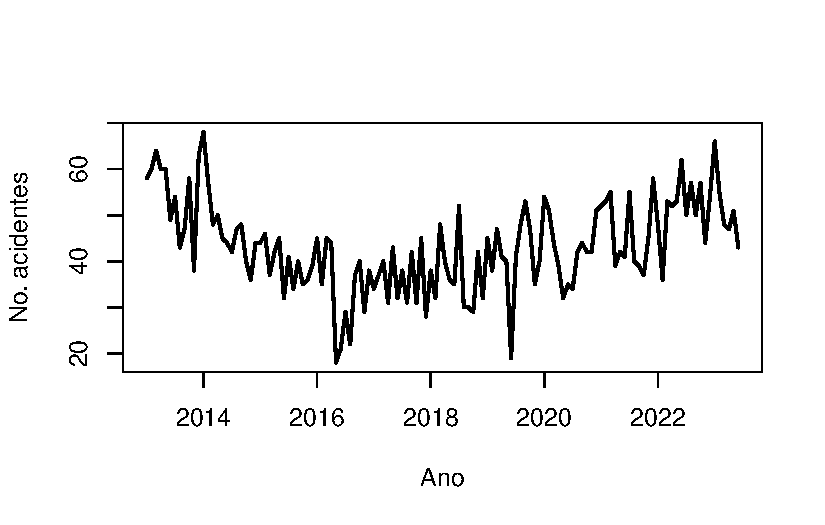
\includegraphics{tendencia_files/figure-pdf/fig-fabMes-1.pdf}

}

\caption{\label{fig-fabMes}Número mensal de acidentes envolvendo
aeronaves. Fonte: FAB}

}

\end{minipage}%

\end{figure}

\hypertarget{tenduxeancia-aletuxf3ria-e-tenduxeancia-determinuxedstica}{%
\section{Tendência aletória e tendência
determinística}\label{tenduxeancia-aletuxf3ria-e-tenduxeancia-determinuxedstica}}

A tendência pode ser duas naturezas: determinística ou aleatória.

A tendência aleatória é construída ao acaso. Considere, por exemplo, o
passeio aleatório definido por \(x_0=0\) e
\(x_t = x_{t-1}+\varepsilon_t\), onde \(\varepsilon_t\) é um ruído
branco gaussiano com \(\nu=1\). Já foi mostrado que \(E(x_t)=0\) e
\(Var(x_t)=t\). A figura abaixo apresenta uma série simulada desse
processo.

\begin{Shaded}
\begin{Highlighting}[]
\FunctionTok{set.seed}\NormalTok{(}\DecValTok{1}\NormalTok{)}
\NormalTok{x }\OtherTok{=} \DecValTok{0}
\ControlFlowTok{for}\NormalTok{( t }\ControlFlowTok{in} \DecValTok{2}\SpecialCharTok{:}\DecValTok{100}\NormalTok{) x[t] }\OtherTok{=}\NormalTok{ x[t }\SpecialCharTok{{-}} \DecValTok{1}\NormalTok{] }\SpecialCharTok{+} \FunctionTok{rnorm}\NormalTok{(}\DecValTok{1}\NormalTok{,}\DecValTok{0}\NormalTok{,}\DecValTok{1}\NormalTok{)}
\FunctionTok{ts.plot}\NormalTok{(x, }\AttributeTok{lwd =} \DecValTok{2}\NormalTok{)}
\end{Highlighting}
\end{Shaded}

\begin{figure}[H]

{\centering 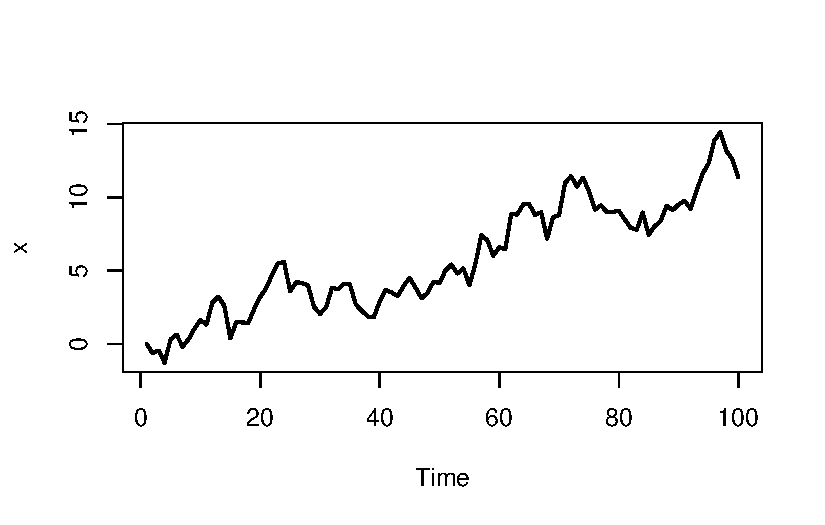
\includegraphics{tendencia_files/figure-pdf/unnamed-chunk-2-1.pdf}

}

\end{figure}

Observe que a série exibe um tendência, mas não há qualquer explicação
para a sua exsitência, uma vez que este comportamento é fruto do acaso.
Ainda, teremos que \(E(x_t)=0\), o que torna o padrão observado
irrelevante.

Na tendência determinística, há uma função T(.) que determina seu
comportamento. Nesse caso, é assumido que

\[y_t = T(t) + \varepsilon_t,\] onde \(\varepsilon_t\) é uma série
estacionária com média \(0\) e variância \(\nu\). Deste modo,
\(E(y_t)=T(t)\), o que implica que \(T(.)\) representa o comportamento
médio da série. O problema de estimar \(T(.)\) é denominado suavização.

Na prática, é impossível determinar se uma tendência é aleatória ou
determinística, cabendo ao estastístico procurar se há motivos para
acreditar que está analisando o segundo tipo. A partir deste momento,
toda tendência será considerada determinística.

\hypertarget{o-modelo-de-tenduxeancia-polinomial}{%
\section{O modelo de tendência
polinomial}\label{o-modelo-de-tenduxeancia-polinomial}}

Considere que a série temporal foi observada até o tempo \(s\). Então, a
tendência é definida como uma função \(T:(0,t]\rightarrow \mathbb{R}\).
O Teorema de Weierstrass afirma que, se \(T\) é contínua, então para
qualquer \(\delta>0\), existe um polinômio \(u(.)\) tal que
\[|T(t)-u(t)|<\delta.\] Isto quer dizer que \(T(.)\) sempre pode ser
aproximada por um polinômio. Assim, para determinada ordem \(p\), é
correto afirmar que\\
\[\begin{equation}
        y_t = \beta_0 + \sum_{j=1}^p \beta_j t^j + \varepsilon_t
        \end{equation}\] onde \(\varepsilon_t\) é uma série
estacionária, é um modelo razoável para uma série temporal com
tendência. Assumindo que \(\varepsilon_t\) é um ruído branco gaussiano,
tem-se o modelo de tendência polinomial de grau \(p\).

Fazendo \(\boldsymbol{f}_t'=(1,t,\ldots,t^p)\) , o modelo de tendência
polinomial é reescrito como
\[\boldsymbol{y}=\boldsymbol{F}'\boldsymbol{\beta}+\boldsymbol{\varepsilon}\]
e inferências sobre \(\boldsymbol{\beta}\) e \(\nu\) são feitas
utilizando o modelo linear tradicional.

\begin{example}[]\protect\hypertarget{exm-nascidos}{}\label{exm-nascidos}

Considere o número anual de nascidos vivos no estado do Amazonas entre
os anos 2000 e 20013:

\begin{Shaded}
\begin{Highlighting}[]
\NormalTok{x }\OtherTok{\textless{}{-}} \FunctionTok{c}\NormalTok{( }\DecValTok{67646}\NormalTok{ , }\DecValTok{70252}\NormalTok{ , }\DecValTok{70671}\NormalTok{ , }\DecValTok{70751}\NormalTok{ , }\DecValTok{71345}\NormalTok{ ,}
        \DecValTok{73488}\NormalTok{ , }\DecValTok{75584}\NormalTok{ , }\DecValTok{73469}\NormalTok{ , }\DecValTok{75030}\NormalTok{ , }\DecValTok{75729}\NormalTok{ , }
        \DecValTok{74188}\NormalTok{ , }\DecValTok{76202}\NormalTok{ , }\DecValTok{77434}\NormalTok{ , }\DecValTok{79041}\NormalTok{)}

\NormalTok{nascidos }\OtherTok{\textless{}{-}} \FunctionTok{ts}\NormalTok{(x, }\AttributeTok{start =}\DecValTok{2000}\NormalTok{)}
\end{Highlighting}
\end{Shaded}

\begin{Shaded}
\begin{Highlighting}[]
\FunctionTok{ts.plot}\NormalTok{(nascidos, }\AttributeTok{lwd =} \DecValTok{2}\NormalTok{, }\AttributeTok{ylab =} \StringTok{\textquotesingle{}No. nascidos vivos\textquotesingle{}}\NormalTok{)}
\NormalTok{stats}\SpecialCharTok{::}\FunctionTok{acf}\NormalTok{(nascidos)}
\end{Highlighting}
\end{Shaded}

\begin{figure}

\begin{minipage}[t]{0.50\linewidth}

{\centering 

\raisebox{-\height}{

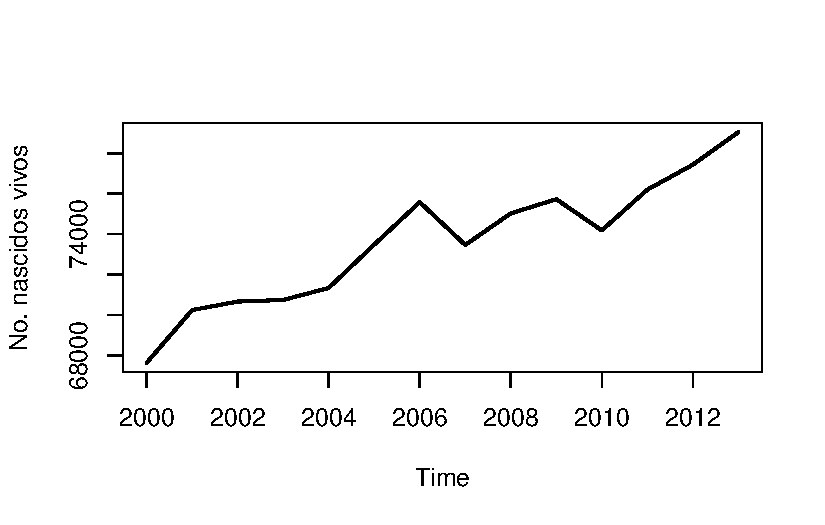
\includegraphics{tendencia_files/figure-pdf/fig-nascidosAM-1.pdf}

}

\caption{\label{fig-nascidosAM-1}Número de nascimentos anual no estado
do Amazonas (Fonte: SINASC/SUS)}

}

\end{minipage}%
%
\begin{minipage}[t]{0.50\linewidth}

{\centering 

\raisebox{-\height}{

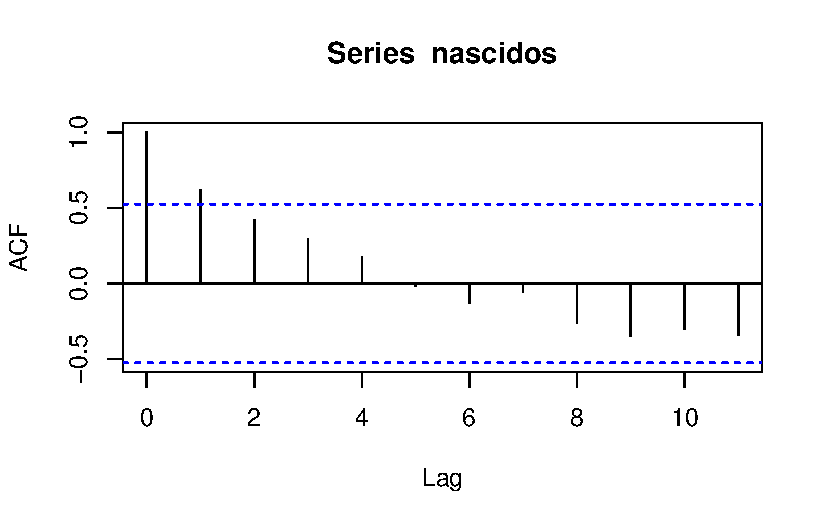
\includegraphics{tendencia_files/figure-pdf/fig-nascidosAM-2.pdf}

}

\caption{\label{fig-nascidosAM-2}Correlograma da série (Fonte:
SINASC/SUS).}

}

\end{minipage}%

\end{figure}

Vamos ajustar um modelo de tendência polinomial de ordem 1, ou seja

\[y_t=\beta_0+\beta_1 t + \varepsilon_t\] onde \(t=1,\ldots,14\)
representa os tempos \(2000,\ldots,2013\).

\begin{Shaded}
\begin{Highlighting}[]
\NormalTok{tempo }\OtherTok{\textless{}{-}} \DecValTok{1}\SpecialCharTok{:}\DecValTok{14}
\NormalTok{mod }\OtherTok{\textless{}{-}} \FunctionTok{lm}\NormalTok{( nascidos }\SpecialCharTok{\textasciitilde{}} \FunctionTok{poly}\NormalTok{(tempo, }\DecValTok{1}\NormalTok{, }\AttributeTok{raw =} \ConstantTok{TRUE}\NormalTok{))}
\end{Highlighting}
\end{Shaded}

As estimativas de máxima verossimilhança para \(\beta_0\) e \(\beta_1\)
são:

\begin{Shaded}
\begin{Highlighting}[]
\NormalTok{mod}\SpecialCharTok{$}\NormalTok{coefficients}
\end{Highlighting}
\end{Shaded}

\begin{verbatim}
               (Intercept) poly(tempo, 1, raw = TRUE) 
                 68266.879                    715.178 
\end{verbatim}

ou seja, \[\hat{T}(t)=\hat{\beta}+\hat{\beta}_1 t = 68.267+715 t\] Os
resíduos do modelo linear \texttt{mod} podem ser obtidos via função
\texttt{residuals}. Abaixo, verificamos que a série dos resíduos oscila
em torno de zero e que nenhuma autocorrelação parece ser relevante, o
que dão indícios de que os erros são um ruído branco.

\begin{Shaded}
\begin{Highlighting}[]
\NormalTok{res }\OtherTok{\textless{}{-}} \FunctionTok{residuals}\NormalTok{(mod)}
\FunctionTok{ts.plot}\NormalTok{( res, }\AttributeTok{main =} \StringTok{\textquotesingle{}\textquotesingle{}}\NormalTok{)}
\FunctionTok{acf}\NormalTok{(res, }\AttributeTok{main =} \StringTok{\textquotesingle{}\textquotesingle{}}\NormalTok{)}
\end{Highlighting}
\end{Shaded}

\begin{figure}

\begin{minipage}[t]{0.50\linewidth}

{\centering 

\raisebox{-\height}{

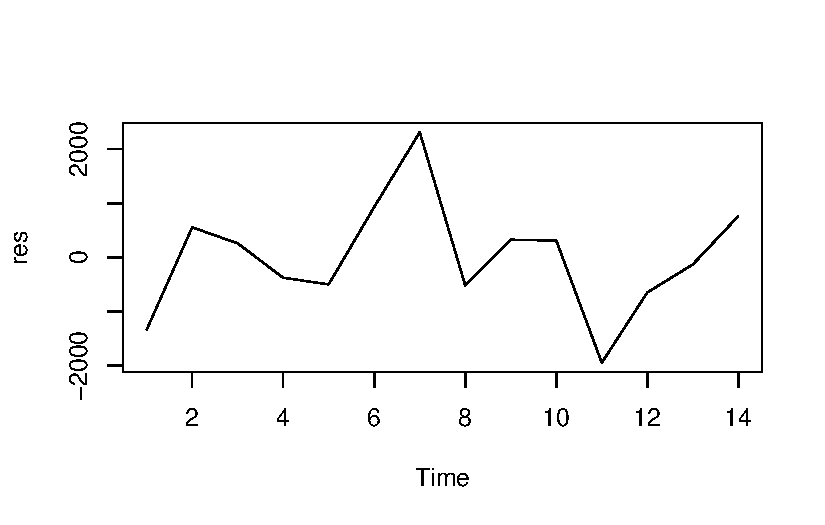
\includegraphics{tendencia_files/figure-pdf/unnamed-chunk-7-1.pdf}

}

\caption{Série dos resíduos}

}

\end{minipage}%
%
\begin{minipage}[t]{0.50\linewidth}

{\centering 

\raisebox{-\height}{

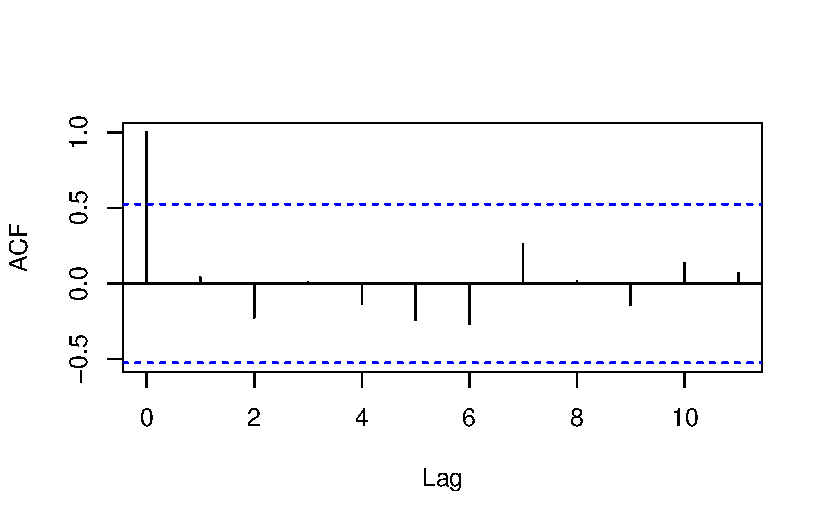
\includegraphics{tendencia_files/figure-pdf/unnamed-chunk-7-2.pdf}

}

\caption{Correlograma dos resíduos}

}

\end{minipage}%

\end{figure}

Abaixo, o teste de Shapiro-Wilks não gera evidências contra a suposição
de normalidade e o teste de Box-Pierce não gera evidências contra a
hipótese de ruído branco.

\begin{Shaded}
\begin{Highlighting}[]
\FunctionTok{shapiro.test}\NormalTok{(res)}
\end{Highlighting}
\end{Shaded}

\begin{verbatim}

    Shapiro-Wilk normality test

data:  res
W = 0.96982, p-value = 0.8743
\end{verbatim}

\begin{Shaded}
\begin{Highlighting}[]
\FunctionTok{Box.test}\NormalTok{(res)}
\end{Highlighting}
\end{Shaded}

\begin{verbatim}

    Box-Pierce test

data:  res
X-squared = 0.02156, df = 1, p-value = 0.8833
\end{verbatim}

É interessante notar que, para \(t=1,\ldots,14\),
\[\hat{T}(t)=\hat{\beta}_0+\hat{\beta}_1 t = \hat{y}_t,\] logo, os
valores preditos do modelo são uma estimativa para a tendência nos
pontos observados.

\begin{Shaded}
\begin{Highlighting}[]
\FunctionTok{ts.plot}\NormalTok{( }\FunctionTok{cbind}\NormalTok{( nascidos, }\FunctionTok{fitted}\NormalTok{(mod)), }\AttributeTok{col =} \DecValTok{1}\SpecialCharTok{:}\DecValTok{2}\NormalTok{, }\AttributeTok{lwd =} \DecValTok{2}\NormalTok{)}
\end{Highlighting}
\end{Shaded}

\begin{figure}

\begin{minipage}[t]{\linewidth}

{\centering 

\raisebox{-\height}{

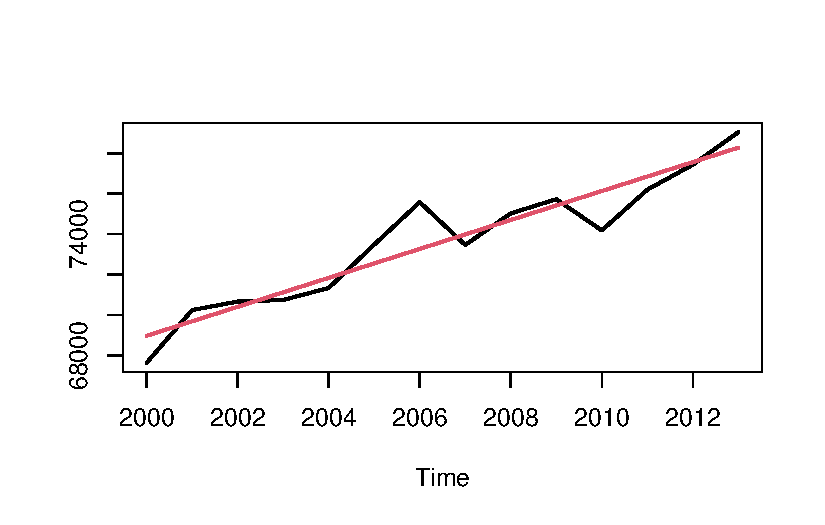
\includegraphics{tendencia_files/figure-pdf/unnamed-chunk-9-1.pdf}

}

\caption{Linha preta: série original. Linha vermelha: tendência
estimada}

}

\end{minipage}%

\end{figure}

\end{example}

\hypertarget{previsuxe3o}{%
\subsection{Previsão}\label{previsuxe3o}}

A previsão é realizada utilizando o modelo ajustado, estrapolando para
um tempo não observado. Por exemplo a estimativa para 2014 (\(t=15\)) é

\[\hat{T}(15)=\hat{\beta}+\hat{\beta}_1 15 = 78.992\] (o valor real foi
81.145).

É importante ressaltar que esse tipo de modelo é interessante para fazer
inferências sobre a tendência, mas pode ser inadequado para previsões,
uma vez que o polinômio é uma aproximação apenas para o intervalo
observado.

\hypertarget{seleuxe7uxe3o-de-modelos-lineares}{%
\subsection{Seleção de modelos
lineares}\label{seleuxe7uxe3o-de-modelos-lineares}}

O valor do Critério de Informação de Akaike (AIC) é dado por
\(-2L(\hat{\theta})+2k\) onde \(L\) é a função de verossimilhança e
\(\hat{\theta}\) e \(k\) são o estimador de máxima verossimilhança para
\(\theta\) e sua dimensão, respectivamente. O modelo com menor AIC é
considerado mais adequado.

Considere o nível anual, em pés, do Lago Huron. Essa série já vem
carregada no \texttt{R} sob o nome \texttt{LakeHuron}.

\begin{Shaded}
\begin{Highlighting}[]
\FunctionTok{ts.plot}\NormalTok{(LakeHuron, }\AttributeTok{lwd =} \DecValTok{2}\NormalTok{, }\AttributeTok{ylab =} \StringTok{\textquotesingle{}Nível (pés)\textquotesingle{}}\NormalTok{)}
\NormalTok{stats}\SpecialCharTok{::}\FunctionTok{acf}\NormalTok{(LakeHuron)}
\end{Highlighting}
\end{Shaded}

\begin{figure}

\begin{minipage}[t]{0.50\linewidth}

{\centering 

\raisebox{-\height}{

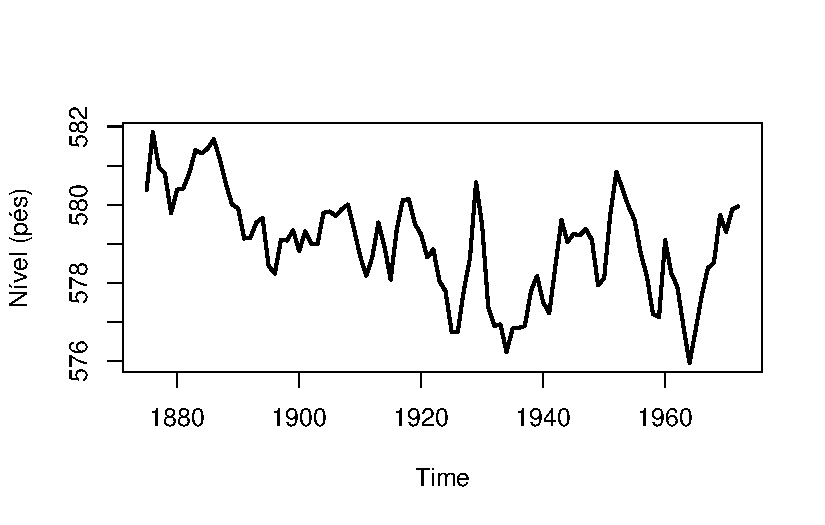
\includegraphics{tendencia_files/figure-pdf/fig-lakeHuron-1.pdf}

}

\caption{\label{fig-lakeHuron-1}Nível anual do Lago Huron, entre 1875 e
1972}

}

\end{minipage}%
%
\begin{minipage}[t]{0.50\linewidth}

{\centering 

\raisebox{-\height}{

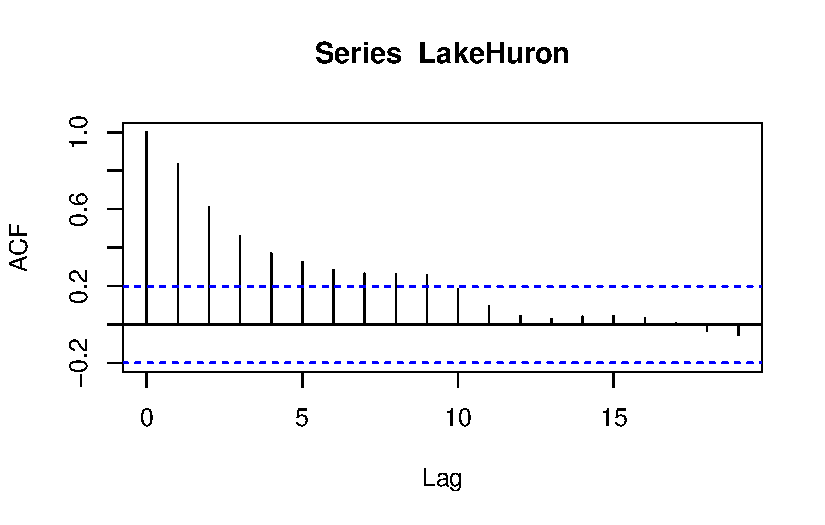
\includegraphics{tendencia_files/figure-pdf/fig-lakeHuron-2.pdf}

}

\caption{\label{fig-lakeHuron-2}Correlograma da série}

}

\end{minipage}%

\end{figure}

Vamos ajustar alguns modelos para tentar explica a tendêndia dessa
série.

\begin{Shaded}
\begin{Highlighting}[]
\NormalTok{tempo }\OtherTok{\textless{}{-}} \DecValTok{1} \SpecialCharTok{:} \FunctionTok{length}\NormalTok{(LakeHuron)}
\NormalTok{mod1 }\OtherTok{\textless{}{-}} \FunctionTok{lm}\NormalTok{( LakeHuron }\SpecialCharTok{\textasciitilde{}} \FunctionTok{poly}\NormalTok{(tempo, }\DecValTok{1}\NormalTok{, }\AttributeTok{raw =}\NormalTok{ T))}
\NormalTok{mod2 }\OtherTok{\textless{}{-}} \FunctionTok{lm}\NormalTok{( LakeHuron }\SpecialCharTok{\textasciitilde{}} \FunctionTok{poly}\NormalTok{(tempo, }\DecValTok{2}\NormalTok{, }\AttributeTok{raw =}\NormalTok{ T))}
\NormalTok{mod3 }\OtherTok{\textless{}{-}} \FunctionTok{lm}\NormalTok{( LakeHuron }\SpecialCharTok{\textasciitilde{}} \FunctionTok{poly}\NormalTok{(tempo, }\DecValTok{3}\NormalTok{, }\AttributeTok{raw =}\NormalTok{ T))}
\NormalTok{mod4 }\OtherTok{\textless{}{-}} \FunctionTok{lm}\NormalTok{( LakeHuron }\SpecialCharTok{\textasciitilde{}} \FunctionTok{poly}\NormalTok{(tempo, }\DecValTok{4}\NormalTok{, }\AttributeTok{raw =}\NormalTok{ T))}
\NormalTok{mod5 }\OtherTok{\textless{}{-}} \FunctionTok{lm}\NormalTok{( LakeHuron }\SpecialCharTok{\textasciitilde{}} \FunctionTok{poly}\NormalTok{(tempo, }\DecValTok{5}\NormalTok{, }\AttributeTok{raw =}\NormalTok{ T))}
\NormalTok{mod6 }\OtherTok{\textless{}{-}} \FunctionTok{lm}\NormalTok{( LakeHuron }\SpecialCharTok{\textasciitilde{}} \FunctionTok{poly}\NormalTok{(tempo, }\DecValTok{6}\NormalTok{, }\AttributeTok{raw =}\NormalTok{ T))}

\FunctionTok{AIC}\NormalTok{(mod1)}
\end{Highlighting}
\end{Shaded}

\begin{verbatim}
[1] 306.0957
\end{verbatim}

\begin{Shaded}
\begin{Highlighting}[]
\FunctionTok{AIC}\NormalTok{(mod2)}
\end{Highlighting}
\end{Shaded}

\begin{verbatim}
[1] 287.8407
\end{verbatim}

\begin{Shaded}
\begin{Highlighting}[]
\FunctionTok{AIC}\NormalTok{(mod3)}
\end{Highlighting}
\end{Shaded}

\begin{verbatim}
[1] 289.8391
\end{verbatim}

\begin{Shaded}
\begin{Highlighting}[]
\FunctionTok{AIC}\NormalTok{(mod4)}
\end{Highlighting}
\end{Shaded}

\begin{verbatim}
[1] 291.7127
\end{verbatim}

\begin{Shaded}
\begin{Highlighting}[]
\FunctionTok{AIC}\NormalTok{(mod5)}
\end{Highlighting}
\end{Shaded}

\begin{verbatim}
[1] 293.475
\end{verbatim}

\begin{Shaded}
\begin{Highlighting}[]
\FunctionTok{AIC}\NormalTok{(mod6)}
\end{Highlighting}
\end{Shaded}

\begin{verbatim}
[1] 291.7054
\end{verbatim}

Entre os modelos ajustados, o de ordem 2 foi aquele com o menor valor do
AIC. Sua tendência estimada é

O polinômio ajustado foi \[\hat{T}(t) = 581 -0,091 t + 0,001 t^2\]

Abaixo, apresentamos a análise de resíduos desse modelo.

\begin{Shaded}
\begin{Highlighting}[]
\NormalTok{res }\OtherTok{\textless{}{-}} \FunctionTok{residuals}\NormalTok{(mod2)}
\FunctionTok{ts.plot}\NormalTok{( res, }\AttributeTok{main =} \StringTok{\textquotesingle{}\textquotesingle{}}\NormalTok{)}
\FunctionTok{abline}\NormalTok{(}\AttributeTok{h =} \DecValTok{0}\NormalTok{, }\AttributeTok{lty =} \DecValTok{2}\NormalTok{)}
\FunctionTok{acf}\NormalTok{(res, }\AttributeTok{main =} \StringTok{\textquotesingle{}\textquotesingle{}}\NormalTok{)}
\end{Highlighting}
\end{Shaded}

\begin{figure}

\begin{minipage}[t]{0.50\linewidth}

{\centering 

\raisebox{-\height}{

\includegraphics{tendencia_files/figure-pdf/unnamed-chunk-12-1.pdf}

}

\caption{Série dos resíduos}

}

\end{minipage}%
%
\begin{minipage}[t]{0.50\linewidth}

{\centering 

\raisebox{-\height}{

\includegraphics{tendencia_files/figure-pdf/unnamed-chunk-12-2.pdf}

}

\caption{Correlograma dos resíduos}

}

\end{minipage}%

\end{figure}

Os resíduos parecem oscilar em torno de zero com um variância constante,
mas o correlograma sugere que não temos um ruído branco. O teste de
Box-Pierce, dado abaixo, confirma a nossa suspeita. Deste modo, este
modelo não é adequado.

\begin{Shaded}
\begin{Highlighting}[]
\FunctionTok{Box.test}\NormalTok{(res)}
\end{Highlighting}
\end{Shaded}

\begin{verbatim}

    Box-Pierce test

data:  res
X-squared = 50.973, df = 1, p-value = 9.365e-13
\end{verbatim}

\hypertarget{muxe9todos-nuxe3o-paramuxe9tricos-para-estimauxe7uxe3o-da-tenduxeancia}{%
\section{Métodos não paramétricos para estimação da
tendência}\label{muxe9todos-nuxe3o-paramuxe9tricos-para-estimauxe7uxe3o-da-tenduxeancia}}

O modelo de tendência polinomial é robusto quando relaxamos a
necessidade do ruído branco ser gaussiano. Nesse sentido, as estimativas
ainda são válidas, mas perdemos todos os testes de hipóteses.

Os métodos não paramétricos independem da distribuição do ruído, sendo
úteis para a análise exploratória.

\hypertarget{muxe9dias-muxf3veis}{%
\subsection{Médias Móveis}\label{muxe9dias-muxf3veis}}

O método das médias móveis consiste em obter \(\hat{T}(t)\) através da
média da série considerando os valores vizinhos à \(y_t\). Para o tempo
\(t\) e \(m=2h+1\), com \(h=1,2,\ldots\), considere o conjunto
\(\mathcal{V}(m)_t=\{t-h,\ldots,t+h\}\). Defini-se a média móvel de
ordem \(m\) (notamção \(m\)-MM) como
\[\hat{T}_h(t)=\frac{1}{m}\sum_{ i = t-h}^{t+h}y_i,\;h<t<n-h\].

Para compreender melhor esse estimador, considere que a relação entre
pontos vizinhos é aproximadamente linear, ou seja, para qualquer
\(t\in\mathcal{V}(m)_t\) existem \(a_\mathcal{V}\) e \(b_\mathcal{V}\)
tais que \[y_t\approx a_\mathcal{V}+b_\mathcal{V}t+\varepsilon_t,\] onde
\(\varepsilon_t\) é considerado uma série temporal estacionária e
ergódica. Então
\[\begin{align}E(\hat{T}(t))&=\frac{a_\mathcal{V}+b_\mathcal{V}(t-h)+\cdots+a_\mathcal{V}+b_\mathcal{V}t+\cdots+a_\mathcal{V}+b_\mathcal{V}(t+h)}{m}\\&=a_\mathcal{V}+b_\mathcal{V}t\end{align}\]
\[Var(\hat{T}(t))=\frac{\nu}{m}+\frac{2}{m}\sum_{j=1}^{2h}j\gamma(j)\]
Observe que, como \(T(.)\) é determinística e os ruídos são
estacionários e ergódicos, então \(Var(\hat{T}(t))\) converge para zero
quando \(m\rightarrow \infty\). Contudo, \(T(.)\) é localmente linear,
logo \(\hat{T}\) é um estimador razoável para valores baixos de \(h\).
Este é um exemplo típico de \emph{trade off} entre víes e variância,
onde não é possível minimizar os dois simultaneamente.

Utilizaremos a função \texttt{ma(x,m)}, do pacote \texttt{forecast} para
encontrar \(m-\)MM para a série `x

\begin{example}[]\protect\hypertarget{exm-NACIDOSMA}{}\label{exm-NACIDOSMA}

Abaixo, apresentamos a série anual histórica de nascidos vivos no
Amazonas desde 1994 até 2021.

\begin{Shaded}
\begin{Highlighting}[]
\NormalTok{x }\OtherTok{\textless{}{-}} \FunctionTok{c}\NormalTok{(}\DecValTok{47780}\NormalTok{, }\DecValTok{47966}\NormalTok{, }\DecValTok{49112}\NormalTok{, }\DecValTok{56070}\NormalTok{, }\DecValTok{57180}\NormalTok{, }\DecValTok{62037}\NormalTok{,}
\DecValTok{67646}\NormalTok{, }\DecValTok{70252}\NormalTok{, }\DecValTok{70671}\NormalTok{, }\DecValTok{70751}\NormalTok{, }\DecValTok{71345}\NormalTok{, }\DecValTok{73488}\NormalTok{, }\DecValTok{75584}\NormalTok{,}
\DecValTok{73469}\NormalTok{, }\DecValTok{75030}\NormalTok{, }\DecValTok{75729}\NormalTok{, }\DecValTok{74188}\NormalTok{, }\DecValTok{76202}\NormalTok{, }\DecValTok{77434}\NormalTok{, }\DecValTok{79041}\NormalTok{,}
\DecValTok{81145}\NormalTok{, }\DecValTok{80097}\NormalTok{, }\DecValTok{76703}\NormalTok{, }\DecValTok{78066}\NormalTok{, }\DecValTok{78087}\NormalTok{, }\DecValTok{77622}\NormalTok{, }\DecValTok{75635}\NormalTok{,}
\DecValTok{78454}\NormalTok{)}

\NormalTok{nascidos }\OtherTok{\textless{}{-}} \FunctionTok{ts}\NormalTok{(x, }\AttributeTok{start =}\DecValTok{1994}\NormalTok{)}
\FunctionTok{ts.plot}\NormalTok{(nascidos, }\AttributeTok{lwd =} \DecValTok{2}\NormalTok{, }\AttributeTok{ylab =} \StringTok{\textquotesingle{}No. nascidos vivos\textquotesingle{}}\NormalTok{)}
\end{Highlighting}
\end{Shaded}

\begin{figure}[H]

{\centering 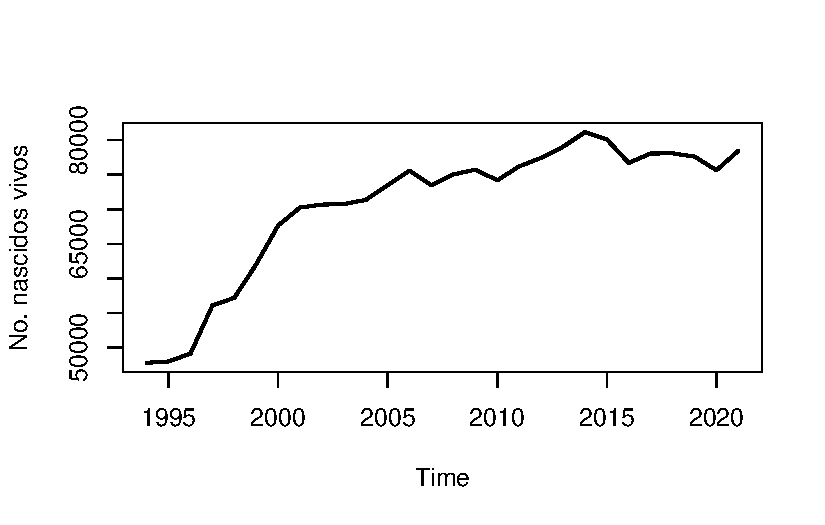
\includegraphics{tendencia_files/figure-pdf/unnamed-chunk-14-1.pdf}

}

\end{figure}

\begin{Shaded}
\begin{Highlighting}[]
\FunctionTok{require}\NormalTok{(forecast)}
\end{Highlighting}
\end{Shaded}

\begin{verbatim}
Carregando pacotes exigidos: forecast
\end{verbatim}

\begin{verbatim}
Warning: package 'forecast' was built under R version 4.3.1
\end{verbatim}

\begin{verbatim}
Registered S3 method overwritten by 'quantmod':
  method            from
  as.zoo.data.frame zoo 
\end{verbatim}

\begin{Shaded}
\begin{Highlighting}[]
\NormalTok{oo }\OtherTok{\textless{}{-}} \FunctionTok{par}\NormalTok{( }\AttributeTok{mfrow =} \FunctionTok{c}\NormalTok{(}\DecValTok{2}\NormalTok{,}\DecValTok{2}\NormalTok{), }\AttributeTok{mar =} \FunctionTok{c}\NormalTok{(}\DecValTok{2}\NormalTok{,}\DecValTok{2}\NormalTok{,}\DecValTok{1}\NormalTok{,}\DecValTok{1}\NormalTok{))}
\FunctionTok{ts.plot}\NormalTok{(nascidos, }\AttributeTok{lwd =} \DecValTok{2}\NormalTok{, }\AttributeTok{ylab =} \StringTok{\textquotesingle{}No. nascidos vivos\textquotesingle{}}\NormalTok{)}
\FunctionTok{lines}\NormalTok{( }\FunctionTok{ma}\NormalTok{(nascidos,}\DecValTok{3}\NormalTok{) , }\AttributeTok{col =}\DecValTok{2}\NormalTok{, }\AttributeTok{lwd =} \DecValTok{2}\NormalTok{)}
\FunctionTok{legend}\NormalTok{(}\StringTok{\textquotesingle{}bottomright\textquotesingle{}}\NormalTok{, }\AttributeTok{legend =} \FunctionTok{c}\NormalTok{(}\StringTok{\textquotesingle{}Série original\textquotesingle{}}\NormalTok{,}\StringTok{\textquotesingle{}3{-}MM\textquotesingle{}}\NormalTok{),  }\AttributeTok{fill =} \FunctionTok{c}\NormalTok{(}\DecValTok{1}\NormalTok{,}\DecValTok{2}\NormalTok{,}\DecValTok{3}\NormalTok{), }\AttributeTok{bty=}\StringTok{\textquotesingle{}n\textquotesingle{}}\NormalTok{)}
\FunctionTok{ts.plot}\NormalTok{(nascidos, }\AttributeTok{lwd =} \DecValTok{2}\NormalTok{, }\AttributeTok{ylab =} \StringTok{\textquotesingle{}No. nascidos vivos\textquotesingle{}}\NormalTok{)}
\FunctionTok{lines}\NormalTok{( }\FunctionTok{ma}\NormalTok{(nascidos,}\DecValTok{5}\NormalTok{) , }\AttributeTok{col =}\DecValTok{2}\NormalTok{, }\AttributeTok{lwd =} \DecValTok{2}\NormalTok{)}
\FunctionTok{legend}\NormalTok{(}\StringTok{\textquotesingle{}bottomright\textquotesingle{}}\NormalTok{, }\AttributeTok{legend =} \FunctionTok{c}\NormalTok{(}\StringTok{\textquotesingle{}Série original\textquotesingle{}}\NormalTok{,}\StringTok{\textquotesingle{}5{-}MM\textquotesingle{}}\NormalTok{),  }\AttributeTok{fill =} \FunctionTok{c}\NormalTok{(}\DecValTok{1}\NormalTok{,}\DecValTok{2}\NormalTok{,}\DecValTok{3}\NormalTok{), }\AttributeTok{bty=}\StringTok{\textquotesingle{}n\textquotesingle{}}\NormalTok{)}
\FunctionTok{ts.plot}\NormalTok{(nascidos, }\AttributeTok{lwd =} \DecValTok{2}\NormalTok{, }\AttributeTok{ylab =} \StringTok{\textquotesingle{}No. nascidos vivos\textquotesingle{}}\NormalTok{)}
\FunctionTok{lines}\NormalTok{( }\FunctionTok{ma}\NormalTok{(nascidos,}\DecValTok{7}\NormalTok{) , }\AttributeTok{col =}\DecValTok{2}\NormalTok{, }\AttributeTok{lwd =} \DecValTok{2}\NormalTok{)}
\FunctionTok{legend}\NormalTok{(}\StringTok{\textquotesingle{}bottomright\textquotesingle{}}\NormalTok{, }\AttributeTok{legend =} \FunctionTok{c}\NormalTok{(}\StringTok{\textquotesingle{}Série original\textquotesingle{}}\NormalTok{,}\StringTok{\textquotesingle{}7{-}MM\textquotesingle{}}\NormalTok{),  }\AttributeTok{fill =} \FunctionTok{c}\NormalTok{(}\DecValTok{1}\NormalTok{,}\DecValTok{2}\NormalTok{,}\DecValTok{3}\NormalTok{), }\AttributeTok{bty=}\StringTok{\textquotesingle{}n\textquotesingle{}}\NormalTok{)}
\FunctionTok{ts.plot}\NormalTok{(nascidos, }\AttributeTok{lwd =} \DecValTok{2}\NormalTok{, }\AttributeTok{ylab =} \StringTok{\textquotesingle{}No. nascidos vivos\textquotesingle{}}\NormalTok{)}
\FunctionTok{lines}\NormalTok{( }\FunctionTok{ma}\NormalTok{(nascidos,}\DecValTok{9}\NormalTok{) , }\AttributeTok{col =}\DecValTok{2}\NormalTok{, }\AttributeTok{lwd =} \DecValTok{2}\NormalTok{)}
\FunctionTok{legend}\NormalTok{(}\StringTok{\textquotesingle{}bottomright\textquotesingle{}}\NormalTok{, }\AttributeTok{legend =} \FunctionTok{c}\NormalTok{(}\StringTok{\textquotesingle{}Série original\textquotesingle{}}\NormalTok{,}\StringTok{\textquotesingle{}9{-}MM\textquotesingle{}}\NormalTok{),  }\AttributeTok{fill =} \FunctionTok{c}\NormalTok{(}\DecValTok{1}\NormalTok{,}\DecValTok{2}\NormalTok{,}\DecValTok{3}\NormalTok{), }\AttributeTok{bty=}\StringTok{\textquotesingle{}n\textquotesingle{}}\NormalTok{)}
\end{Highlighting}
\end{Shaded}

\begin{figure}[H]

{\centering 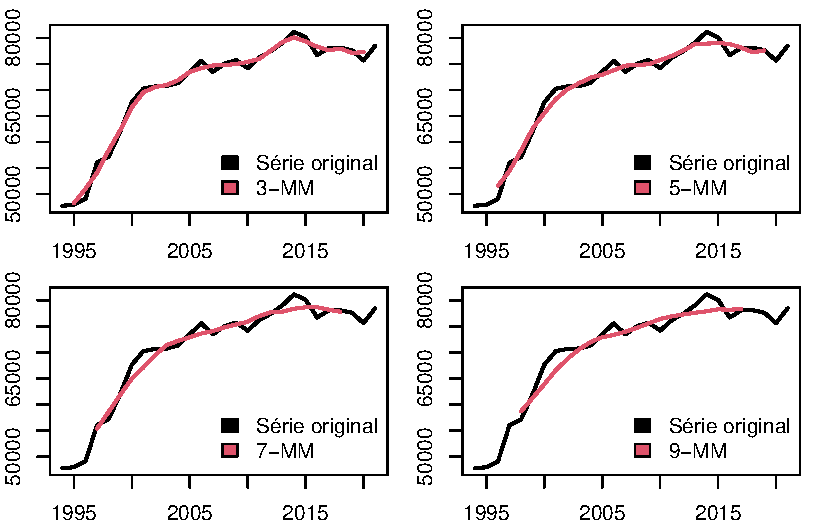
\includegraphics{tendencia_files/figure-pdf/unnamed-chunk-15-1.pdf}

}

\end{figure}

\begin{Shaded}
\begin{Highlighting}[]
\FunctionTok{par}\NormalTok{(oo)}
\end{Highlighting}
\end{Shaded}

Considere a estimativa obtida pela média móvel de ordem 3.

\begin{Shaded}
\begin{Highlighting}[]
\NormalTok{tendencia }\OtherTok{\textless{}{-}} \FunctionTok{ma}\NormalTok{(nascidos, }\DecValTok{3}\NormalTok{)}
\NormalTok{tendencia}
\end{Highlighting}
\end{Shaded}

\begin{verbatim}
Time Series:
Start = 1994 
End = 2021 
Frequency = 1 
 [1]       NA 48286.00 51049.33 54120.67 58429.00 62287.67 66645.00 69523.00
 [9] 70558.00 70922.33 71861.33 73472.33 74180.33 74694.33 74742.67 74982.33
[17] 75373.00 75941.33 77559.00 79206.67 80094.33 79315.00 78288.67 77618.67
[25] 77925.00 77114.67 77237.00       NA
\end{verbatim}

Vamos estimar o ruído da série (e eliminar as coordenadas vazias)

\begin{Shaded}
\begin{Highlighting}[]
\NormalTok{ruido }\OtherTok{\textless{}{-}}\NormalTok{ nascidos }\SpecialCharTok{{-}}\NormalTok{ tendencia}
\NormalTok{ruido }\OtherTok{\textless{}{-}}\NormalTok{ ruido[}\FunctionTok{is.na}\NormalTok{(ruido) }\SpecialCharTok{==}\NormalTok{ F]}
\end{Highlighting}
\end{Shaded}

Abaixo, apresentamos as principais estatísticas sobre os resíduos. A
série histórica dos resíduos oscila em torno de zero e não há motivos
para suspeitar de que sua variância é constante. O correlograma
apresenta autocorrelações baixas, como o esperado em um ruído branco. O
teste de Shapiro-Wilks não dá evidências contra normalidade, o que
suporta a hipótese de ruído branco gaussiano. O teste de Box-Pierce
apresenta um p-valor de 0,04 e, em conjunto com as demais evidências,
vamos considerá-lo significativo ao nível de 4\%.

\begin{Shaded}
\begin{Highlighting}[]
\FunctionTok{ts.plot}\NormalTok{(ruido)}
\FunctionTok{abline}\NormalTok{( }\AttributeTok{h =} \DecValTok{0}\NormalTok{, }\AttributeTok{lty =} \DecValTok{2}\NormalTok{)}
\FunctionTok{abline}\NormalTok{( }\AttributeTok{h =} \DecValTok{2}\SpecialCharTok{*}\FunctionTok{sd}\NormalTok{(ruido), }\AttributeTok{lty=}\DecValTok{2}\NormalTok{)}
\FunctionTok{abline}\NormalTok{( }\AttributeTok{h =} \SpecialCharTok{{-}}\DecValTok{2}\SpecialCharTok{*}\FunctionTok{sd}\NormalTok{(ruido), }\AttributeTok{lty=}\DecValTok{2}\NormalTok{)}
\end{Highlighting}
\end{Shaded}

\begin{figure}[H]

{\centering 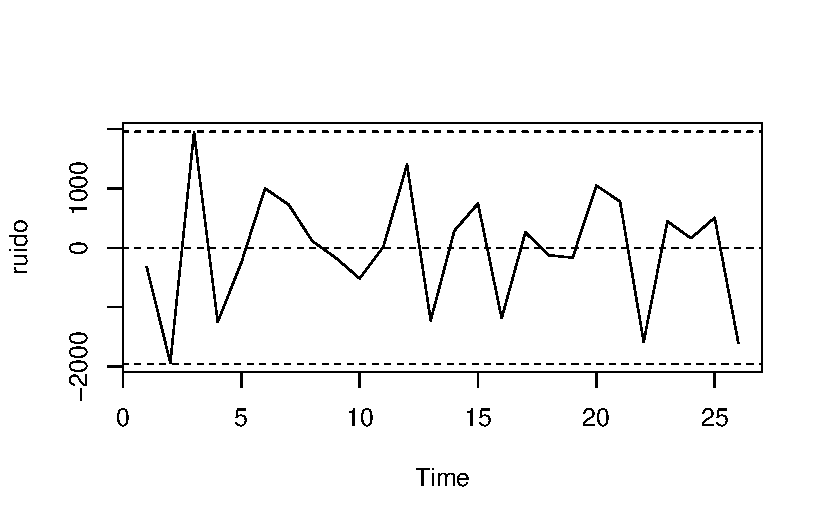
\includegraphics{tendencia_files/figure-pdf/unnamed-chunk-18-1.pdf}

}

\end{figure}

\begin{Shaded}
\begin{Highlighting}[]
\FunctionTok{acf}\NormalTok{(ruido)}
\end{Highlighting}
\end{Shaded}

\begin{figure}[H]

{\centering 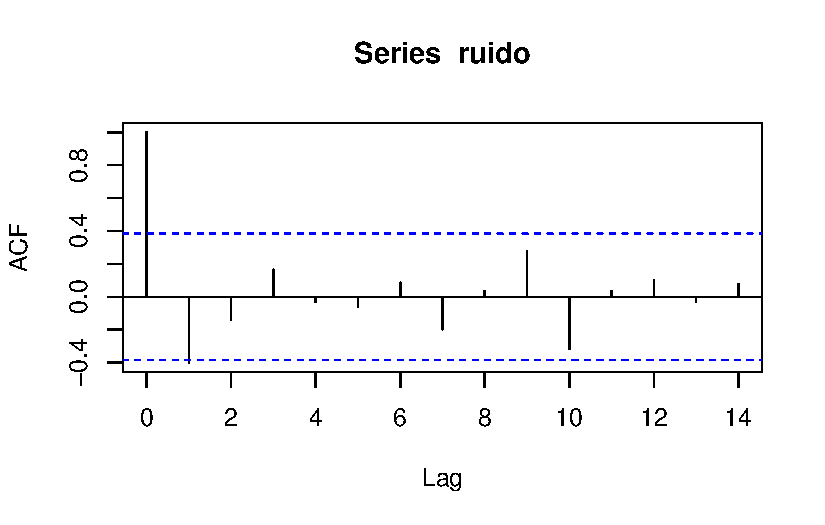
\includegraphics{tendencia_files/figure-pdf/unnamed-chunk-18-2.pdf}

}

\end{figure}

\begin{Shaded}
\begin{Highlighting}[]
\FunctionTok{shapiro.test}\NormalTok{(ruido)}
\end{Highlighting}
\end{Shaded}

\begin{verbatim}

    Shapiro-Wilk normality test

data:  ruido
W = 0.9711, p-value = 0.6521
\end{verbatim}

\begin{Shaded}
\begin{Highlighting}[]
\FunctionTok{Box.test}\NormalTok{(ruido)}
\end{Highlighting}
\end{Shaded}

\begin{verbatim}

    Box-Pierce test

data:  ruido
X-squared = 4.1804, df = 1, p-value = 0.04089
\end{verbatim}

\(\blacksquare\)

\end{example}

Até o momento, foi considerado que a ordem da média móvel é escrita como
\(m=2h+1\), ou seja, a ordem é sempre ímpar. Sem Para definir a média
móvel para uma ordem par, perda de generalidade, assuma que \(m=4\).
Como não é possível escolher um número igual de vizinhos à \(y_t\),
tem-se duas possibilidades para \(\mathcal{V}(4)_t\):
\[\mathcal{V}'(4)_t=\{y_{t-1},y_t,y_{t+1},y_{t+2}\}\] e
\[\mathcal{V}''(4)_t=\{y_{t-2},y_{t-1},y_t,y_{t+1}\}.\] Para cada
possibilidade, tem-se \[\hat{T}'(t)=\frac{1}{4}\sum_{i=t-1}^{t+2}y_{i}\]
e \[\hat{T}''(t)=\frac{1}{4}\sum_{i=t-2}^{t+1}y_{i}.\] A média móvel
2-MM será definida por \[\hat{T}(t)=\frac{T'(t)+T''(t)}{2}\] Observe que
a média agora é ponderada, uma vez que

\[\hat{T}(t)=\frac{y_{t-2}}{8}+\frac{y_{t-1}}{4}+\frac{y_{t}}{4}+\frac{y_{t+1}}{4}+\frac{y_{t+2}}{8}.\]

Para o caso de \(m=2h\) com \(h=1,2,\ldots\), defini-se \(m\)-MM por
\[\begin{align}\hat{T}(t)&=\frac{1}{2}\left[\frac{1}{m}\sum_{i=t-h}^{t+h-1}y_i+\frac{1}{m}\sum_{i=t-h+1}^{t+h}y_i\right]\\&=\frac{y_{t-h}}{2m}+\frac{1}{m}\sum_{i=t-h+1}^{t+h-1}y_i+\frac{y_{t+h}}{2m}.\end{align}\]
Note que o argumento de \(\hat{T}(t)\) é aproximadamente não viciado
para \(m\) pequeno não se altera, uma vez que os pesos para os tempos
\(t-j\) e \(t+j\) são simétricos

O estimador para tendência conhecido como média móvel ponderada de ordem
\(m\) é dado por

\[\hat{T}(t)=\sum_{i=t-h}^{t+h} w_i y_{i},\] com \(w_i>0\),
\(w_{t-j}=w_{t+j}\) e \(\sum_{i=t-h}^{t+h}w_i=1\). O método tradicional
é obtido fazendo \(w_i=1/m\).

Por último, como as primeiras e últimas observações são removidas, esses
métodos não são os mais recomendados.

\textbf{Outras médias móveis}

É importante ressaltar que os métodos estatísticos são ferramentas
universais e que geralmente sofrem modificações ao serem aplicados em
outras áreas. Deste modo, existem outras definições de médias móveis que
podem causar confusão.

Em epidemiologia por exemplo, a média móvel de ordem \(m\) é definida
por \[\hat{T}(t)=\frac{1}{m}\sum_{j=1}^m y_{t-j+1}\] ou seja, a soma dos
valores mais recentes em relação à \(t\). Observe que o contexto é
diferente: em uma epidemia por exemplo, deseja-se estimar \(T(t)\) onde
\(t\) é o tempo mais recente e, em geral, se utiliza o 7-MM tirando a
média dos últimos 7 dias. A mesma lógica vale para o mercado financeiro,
que tira a média dos últimos 5 dias de preço de fechamento.

Ainda no mercado financeiro, o importante é captar a mudança da
tendência o mais rápido possível. Deste modo, utiliza-se uma média móvel
ponderada definida por
\[\hat{T}(t)=\frac{2}{m(m+1)}\sum_{j=1}^m(m-j+1)y_{t-j+1}.\] Na
definição acima, o último preço da ação, dado por \(y_t\), é o valor
mais imporante e por isso recebe o maior peso. Note que os pesos não são
simétricos.

\hypertarget{suavizauxe7uxe3o-do-gruxe1fico-de-dispersuxe3o-estimada-localmente-loess}{%
\section{Suavização do gráfico de dispersão estimada localmente
(loess)}\label{suavizauxe7uxe3o-do-gruxe1fico-de-dispersuxe3o-estimada-localmente-loess}}

No método de suavisação do gráfico de dispersão, deseja-se estimar
\(f(x)=E(y|x)\), através da coleção \((y_1,x_1),\ldots,(y_n,x_n)\), para
um valor qualquer de \(x\).

A estimativa \(\hat{f}\) para o ponto \(x'\) é calculada considerando os
seguintes passos:

\begin{enumerate}
\def\labelenumi{\arabic{enumi}.}
\item
  Fixe um valor inteiro positivo \(q\leq n\).
\item
  Dentro do conjunto \(x_1,\ldots,x_n,\) encontre os \(q\) valores mais
  próximos de \(x'\) (via distância euclidiana). Denote este conjunto
  por \(\mathcal{V}\) e denote por \(d\) a maior distância encontrada.
\item
  Para cada \(x_1,\ldots,x_n\) seja
  \[v_j(x')=\left\{\begin{array}{ll}\left(1-\left| \frac{x_j-x'}{d}\right|^3\right)^3&,\;\;\hbox{se }|x_j-x|\leq d\\ 0,&\hbox{caso contrário}\end{array}\right.\]
  o peso associado à \(x_j\) (valores próximos de \(x'\) receberão o
  peso máximo e valores afastados recebem menor peso)
\item
  Ajuste o modelo de regressão ponderado, minimizando
  \[\sum_{i=1}^n v_i(x')\left(y_i - \sum_{j=0}^p \beta_jx^j\right)^2\]
\item
  Estime \(f(x')\) por \[\hat{f}(x')=\sum_{j=0}^p \hat{\beta}_jx^j \]
\end{enumerate}

Oberve que este método pode ser utilizado para estimar a tendência da
série. Abaixo, vamos analisar a série de taxa de desemprego mensal,
entre março de 2002 e dezembro de 2015.

\begin{Shaded}
\begin{Highlighting}[]
\NormalTok{url }\OtherTok{\textless{}{-}} \StringTok{\textquotesingle{}https://www.dropbox.com/s/rmgymzsic99qawd/desemprego.csv?dl=1\textquotesingle{}}

\NormalTok{banco }\OtherTok{\textless{}{-}} \FunctionTok{read.csv}\NormalTok{(url, }\AttributeTok{sep =} \StringTok{\textquotesingle{};\textquotesingle{}}\NormalTok{, }\AttributeTok{h =}\NormalTok{ F)}

\NormalTok{desemprego}\OtherTok{\textless{}{-}} \FunctionTok{ts}\NormalTok{( banco}\SpecialCharTok{$}\NormalTok{V2, }\AttributeTok{start =} \FunctionTok{c}\NormalTok{(}\DecValTok{2002}\NormalTok{,}\DecValTok{3}\NormalTok{), }\AttributeTok{frequency=}\DecValTok{12}\NormalTok{)}

\FunctionTok{ts.plot}\NormalTok{(desemprego, }\AttributeTok{ylab =} \StringTok{\textquotesingle{}Taxa de desemprego\textquotesingle{}}\NormalTok{)}
\end{Highlighting}
\end{Shaded}

\begin{figure}[H]

{\centering 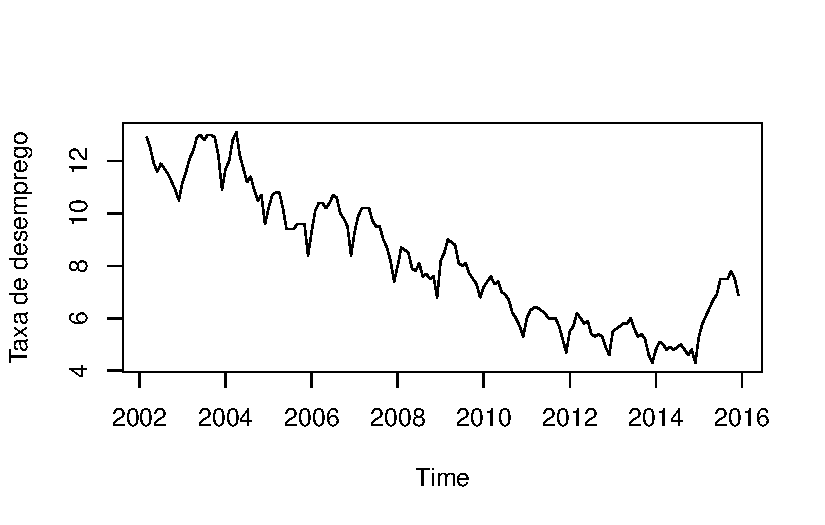
\includegraphics{tendencia_files/figure-pdf/unnamed-chunk-19-1.pdf}

}

\end{figure}

\begin{Shaded}
\begin{Highlighting}[]
\FunctionTok{acf}\NormalTok{(desemprego, }\AttributeTok{lag =} \DecValTok{30}\NormalTok{)}
\end{Highlighting}
\end{Shaded}

\begin{figure}[H]

{\centering 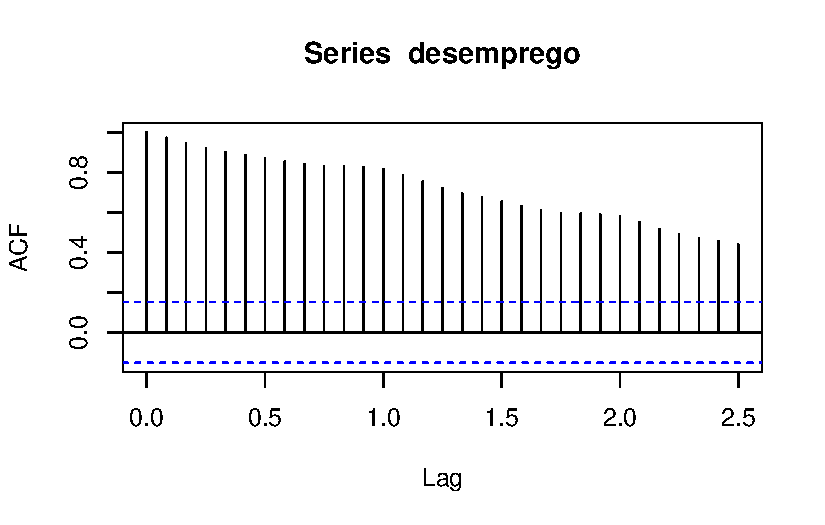
\includegraphics{tendencia_files/figure-pdf/unnamed-chunk-19-2.pdf}

}

\end{figure}

Vamos estimar a tendência

\begin{Shaded}
\begin{Highlighting}[]
\CommentTok{\# criando a variável regressora}
\NormalTok{tempo }\OtherTok{\textless{}{-}} \DecValTok{1} \SpecialCharTok{:} \FunctionTok{length}\NormalTok{(desemprego)}

\CommentTok{\# aplicando o loess}
\NormalTok{lw }\OtherTok{\textless{}{-}} \FunctionTok{loess}\NormalTok{( desemprego }\SpecialCharTok{\textasciitilde{}}\NormalTok{ tempo)}

\CommentTok{\# transformando o valor predito em uma série temporal}

\NormalTok{fit }\OtherTok{\textless{}{-}} \FunctionTok{ts}\NormalTok{(lw}\SpecialCharTok{$}\NormalTok{fitted, }\AttributeTok{start =} \FunctionTok{start}\NormalTok{(desemprego), }\AttributeTok{frequency =} \FunctionTok{frequency}\NormalTok{(desemprego) )}

\CommentTok{\# gráfico da tendência estimada}

\FunctionTok{ts.plot}\NormalTok{( desemprego, }\AttributeTok{ylab =} \StringTok{\textquotesingle{}Taxa de desemprego\textquotesingle{}}\NormalTok{ , }\AttributeTok{lwd =} \DecValTok{2}\NormalTok{)}
\FunctionTok{lines}\NormalTok{(fit, }\AttributeTok{lwd =} \DecValTok{2}\NormalTok{, }\AttributeTok{col =} \StringTok{\textquotesingle{}tomato\textquotesingle{}}\NormalTok{)}
\FunctionTok{legend}\NormalTok{(}\StringTok{\textquotesingle{}topright\textquotesingle{}}\NormalTok{, }\FunctionTok{c}\NormalTok{(}\StringTok{\textquotesingle{}Observado\textquotesingle{}}\NormalTok{,}\StringTok{\textquotesingle{}Ajustado\textquotesingle{}}\NormalTok{),}\AttributeTok{fill=}\FunctionTok{c}\NormalTok{(}\DecValTok{1}\NormalTok{,}\StringTok{\textquotesingle{}tomato\textquotesingle{}}\NormalTok{), }\AttributeTok{bty=}\StringTok{\textquotesingle{}n\textquotesingle{}}\NormalTok{)}
\end{Highlighting}
\end{Shaded}

\begin{figure}[H]

{\centering 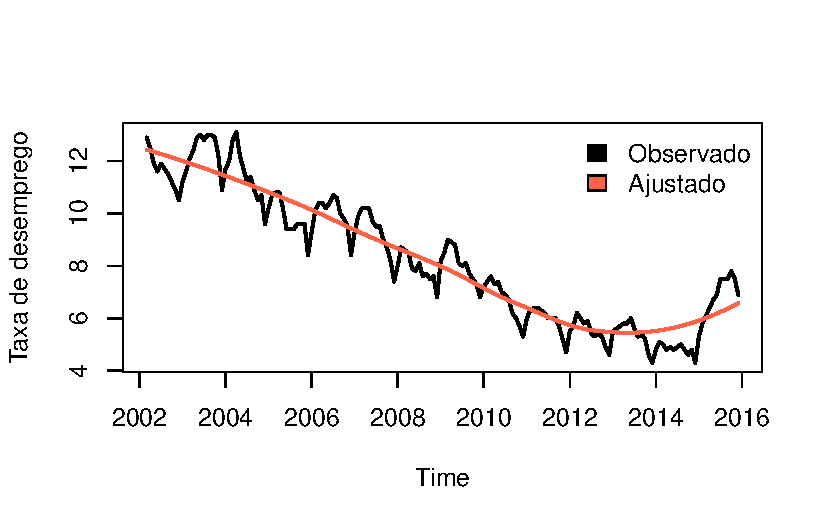
\includegraphics{tendencia_files/figure-pdf/unnamed-chunk-20-1.pdf}

}

\end{figure}

Vamos eliminar a tendência estimada e avaliar o restante.

\begin{Shaded}
\begin{Highlighting}[]
\NormalTok{yt }\OtherTok{\textless{}{-}}\NormalTok{ desemprego }\SpecialCharTok{{-}}\NormalTok{ fit}

\FunctionTok{ts.plot}\NormalTok{(yt)}
\end{Highlighting}
\end{Shaded}

\begin{figure}[H]

{\centering 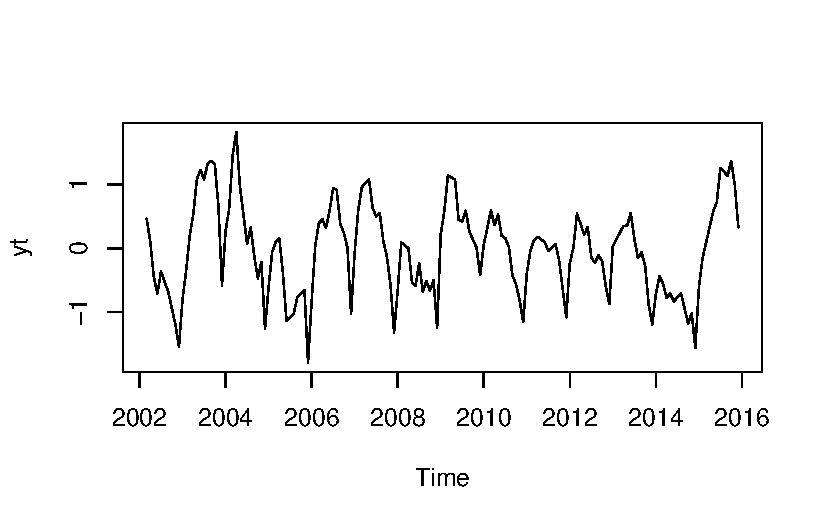
\includegraphics{tendencia_files/figure-pdf/unnamed-chunk-21-1.pdf}

}

\end{figure}

\begin{Shaded}
\begin{Highlighting}[]
\FunctionTok{acf}\NormalTok{(yt)}
\end{Highlighting}
\end{Shaded}

\begin{figure}[H]

{\centering 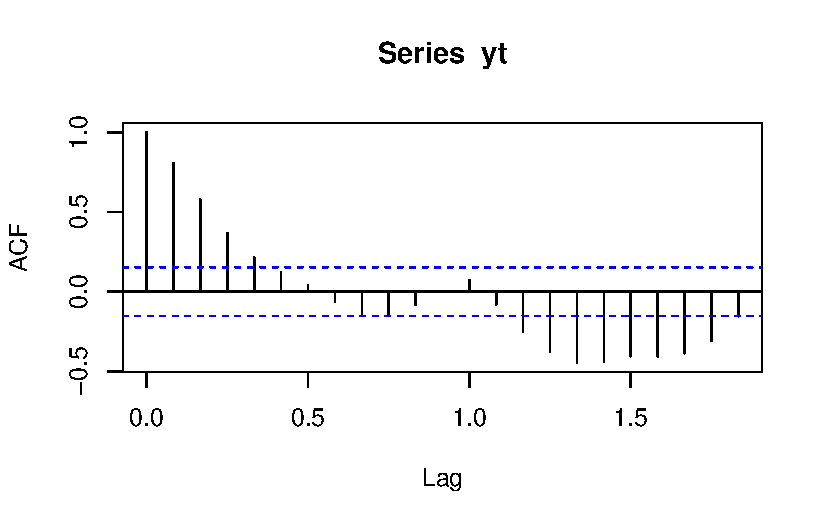
\includegraphics{tendencia_files/figure-pdf/unnamed-chunk-21-2.pdf}

}

\end{figure}

Fica claro o comportamento sazonal, o que implica que o restante não é
uma série estacionária.

\bookmarksetup{startatroot}

\hypertarget{references}{%
\chapter*{References}\label{references}}
\addcontentsline{toc}{chapter}{References}

\markboth{References}{References}

\hypertarget{refs}{}
\begin{CSLReferences}{0}{0}
\end{CSLReferences}



\end{document}
